\documentclass[11pt]{article}
\usepackage[T1]{fontenc}
\usepackage[utf8]{inputenc}
\usepackage[margin=1in]{geometry}
\usepackage{amsmath,amsthm,mathtools}
\usepackage{newpxtext,newpxmath}
\usepackage{microtype}
\usepackage{booktabs,tabularx,array}
\usepackage{enumitem}
\usepackage{xcolor}
\usepackage{tikz}
\usetikzlibrary{arrows.meta,patterns}
\usepackage[numbers,sort&compress]{natbib}
\usepackage[colorlinks=true,linkcolor=blue!45!black,citecolor=blue!45!black,
  urlcolor=blue!45!black]{hyperref}
\usepackage{bookmark}
\hypersetup{pdftitle={Understanding Nondeterminism: Faster SAT and Exact Counting for Small Circuits},
  pdfauthor={Samuel Schlesinger},
  pdfsubject={Restricted-instance SAT algorithms and circuit nondeterminism}}
\usepackage{fancyhdr}
\pagestyle{fancy}
\fancyhf{}
\fancyhead[L]{\small Understanding nondeterminism}
\fancyhead[R]{\small Working manuscript}
\fancyfoot[C]{\thepage}
\setlength{\headheight}{14pt}
\setlength{\emergencystretch}{1.5em}
\setlist{itemsep=3pt,topsep=5pt}
\newtheorem{theorem}{Theorem}[section]
\newtheorem{proposition}[theorem]{Proposition}
\newtheorem{lemma}[theorem]{Lemma}
\newtheorem{corollary}[theorem]{Corollary}
\theoremstyle{definition}
\newtheorem{definition}[theorem]{Definition}
\newtheorem{question}[theorem]{Open question}
\theoremstyle{remark}
\newtheorem{remark}[theorem]{Remark}
\newcommand{\B}{\{0,1\}}
\newcommand{\C}{\mathrm{C}}
\newcommand{\NP}{\mathsf{NP}}
\newcommand{\Ppoly}{\mathsf{P}/\mathrm{poly}}
\newcommand{\poly}{\operatorname{poly}}
\newcommand{\OR}{\bigvee}
\newcommand{\AND}{\bigwedge}
\newcommand{\E}{\mathbb{E}}
\newcommand{\Prb}{\mathbb{P}}
\DeclareMathOperator{\fanin}{fanin}
\DeclareMathOperator{\fanout}{fanout}

\title{Understanding Nondeterminism:\\
  Faster SAT and Exact Counting\\
  for Small Circuits}
\author{Samuel Schlesinger}
\date{September 5, 2026}

\begin{document}
\maketitle
\vspace{-1.5em}
\begin{abstract}
We derive a SAT and exact-counting algorithm that beats exhaustive
search for single-output Boolean circuits with $u$ inputs and
$s\le(4-\gamma)u$ gates, for every fixed $0<\gamma<4$, over the
full binary basis $B_2$ with unrestricted fan-out. For each fixed
$\varepsilon>0$, its running time is
$\poly_\varepsilon(s+u+1)2^{(1/4+\varepsilon)(s+1)}$, allowing
exponential space. The sharper exponent is
$\min\{b,(1/3+\delta)(s+1-b)\}$ for fixed $\delta>0$, where $b$
counts the inputs in a normalized output cone. The proof encodes
consistent circuit values as tables, preserves exact counts through
cubic reduction, and combines the Fomin--H\o ie pathwidth theorem
with frontier contraction and input enumeration.

The same consistency budget explains when existential projection
$g(x)=\exists y\,f(x,y)$ has a small deterministic circuit.
For an $s$-gate verifier, we prove
$\C(g)=O_\varepsilon((s+1)2^{(1/5+\varepsilon)(s+1)})$.
We derive necessary structure for near-full amplification at the
critical gate budget and realize nearly critical supplied budgets
with easy projections, exposing the role of nonminimal verifiers.
A joint witness-sampling and shared-computation bound gives further
improvements, illustrated by analytical families.

The algorithmic improvement is over exhaustive search on the stated
restricted instances. Historical priority and best-known
unrestricted-space status of the precise bound remain unestablished.
The full counting algorithm is not implemented or benchmarked here;
the methods appendix records the AI-assisted workflow and the finite
checks of supporting constructions.
\end{abstract}

\clearpage
\setcounter{tocdepth}{1}
\tableofcontents
\clearpage

\section{SAT and exact counting below four gates per input}
\label{sec:algorithm-overview}

The algorithmic entry point is a restricted-instance improvement over
exhaustive search. Let $C$ be a single-output Boolean circuit with $u$
input bits and $s$ internal gates. Work over the full binary basis $B_2$:
every Boolean function of at most two inputs is a unit-cost gate,
constants and wiring are free, and fan-out is unrestricted.

The construction exploits two complementary measures: the number of
used inputs and the size of the boundary needed to maintain consistency.
The worked example establishes the local mechanism for summarizing a
region by conditional counts. The general argument separates exactness
of these summaries from the existence of an efficiently constructed
narrow processing order. The counting invariant establishes correctness;
the graph theorem supplies the resource bound.

\paragraph{Headline guarantee.}
For every fixed $\varepsilon>0$, the construction counts the satisfying
assignments of $C$, and therefore decides its satisfiability, in time
\begin{equation}\label{eq:headline-sat}
 \boxed{\quad
 \poly_\varepsilon(s+u+1)\,
 2^{(1/4+\varepsilon)(s+1)}.
 \quad}
\end{equation}
The space bound allows the same exponential factor. Consequently, for
each fixed $0<\gamma<4$, circuits with $s\le(4-\gamma)u$ admit an
algorithm running in $\poly_\gamma(u)2^{(1-\eta)u}$ for some
$\eta>0$ depending only on $\gamma$. This beats the $2^u$ enumeration
bound by an exponential factor. The restriction concerns the gate
budget in $B_2$, not the number of clauses in a CNF representation.

For example, take $\varepsilon=\gamma/[8(4-\gamma)]$ in
\eqref{eq:headline-sat}. Then
\[
 (1/4+\varepsilon)(s+1)
 \le (1-\gamma/8)u+(1/4+\varepsilon),
\]
so $\eta=\gamma/8$ is an explicit choice. The additive constant is
absorbed into the prefactor. The positive slack is fixed before the
input size grows; no exact endpoint exponent with a fixed polynomial
prefactor is asserted.

\paragraph{Why the running time improves.}
Normalize the output cone without changing its function, leaving $b$
used inputs. Each removed input contributes a factor of two to the
final count. Encode the circuit's gate equations, consistent uses of
every input and gate value, and the requirement that its output is one
as a network of small tables. Every satisfying input assignment has
exactly one extension to the internal values. The network's cycle rank
$\kappa$ satisfies
\[
 \kappa\le s+1-b.
\]
Split high-degree equality tables into trees, then contract low-degree
parts, loops, and parallel edges with exact table identities. A
nonempty residual simple cubic graph has at most $2(\kappa-1)$
vertices. The constructive Fomin--H\o ie theorem
\citep{FominHoie2006}, together with the width conversion proved below,
gives a vertex order with at most $(1/3+\delta)\kappa+O_\delta(1)$
edges crossing any frontier. Summing over the frontier assignments
evaluates the network using integer addition and multiplication.
Intermediate counts have polynomial bit length.

Choosing between this contraction and enumeration of the $b$ used
inputs gives the sharper bound
\begin{equation}\label{eq:headline-sensitive}
 \poly_\delta(s+u+1)\,
 2^{\min\{b,(1/3+\delta)(s+1-b)\}},
 \qquad \delta>0\text{ fixed}.
\end{equation}
Writing $\alpha=1/3+\delta$, the two exponents balance at
$b=\alpha(s+1)/(1+\alpha)$, where their common value is
$\alpha(s+1)/(1+\alpha)$. Its gate coefficient approaches $1/4$.
Section~\ref{sec:consistency-graph} proves the graph construction,
reductions, and frontier bound; Corollary~\ref{cor:gate-counting}
proves the uniform count-preserving algorithm and its bit complexity.

\paragraph{Status and scope.}
This is an asymptotic algorithm with exponential space, derived from
established width and tensor methods with explicit circuit-specific
accounting. The repository contains finite checks of supporting
constructions and a Rust implementation of the complete automatic
counting route in \texttt{rs/}. Its source-to-proof correspondence and
fixed-parameter resource argument are recorded in \texttt{rs/ALGORITHM.md}.
The retained structured timings illustrate a mechanism; they do not
establish the asymptotic bound empirically. Historical priority of the precise bound and its
best-known unrestricted-space status remain unestablished; the
statement-level comparison is in Section~\ref{sec:prior-work}.

\paragraph{From SAT to understanding nondeterminism.}
The proof first asks what changes when only witness inputs
are quantified and ordinary inputs remain symbolic. The same
consistency budget then gives a nonuniform circuit-size exponent
approaching $1/5$, alongside witness-coverage bounds, necessary
conditions for strong amplification, and examples separating a
complicated supplied circuit from an intrinsically hard function.

Returning to integer tables then gives the SAT bound and its consequences
for search, indexing, and exact generation in
Section~\ref{sec:algorithm-consequences}.


\section{The question and its quantifiers}

We study
\[
 f:\B^{n+m}\longrightarrow\B,
 \qquad
 g(x)=\OR_{y\in\B^m}f(x,y).
\]
Circuit complexity measures the size of the \emph{smallest} circuit for
a function. It does not measure the cost of discovering that circuit.
In particular, a circuit for $g$ may exploit facts about $f$ that are
expensive to discover algorithmically.

\paragraph{Model.}
Unless explicitly stated otherwise, circuits are finite directed acyclic
graphs over the full binary basis $B_2$: every Boolean operation of at
most two inputs is available at unit cost. Constants and input/output
wiring are free; fan-out is unrestricted. The number of internal gates
is the size. Write $\C(h)$ for minimum size and
\[
 M_n=\max_{h:\B^n\to\B}\C(h).
\]
Changing to any fixed complete bounded-fan-in basis changes size by
constant factors. Exact constants in gate-counting results, including
the limiting coefficient $1/5$ in our size-dependent exponent, are basis-specific.
All logarithms are base two, except $\ln$. Comparisons with $2^n/n$
assume $n\ge2$.

\begin{definition}[Worst-case projection complexity]
For nonnegative integers $n,m,s$, let
\[
 D(n,m,s)=\max\left\{\C(\exists y\,f(x,y)):
                 f:\B^{n+m}\to\B,\ \C(f)\le s\right\}.
\]
Equivalently, if $N_m(h)$ is the minimum complexity of a verifier for
$h$ using at most $m$ witness bits, then
$D(n,m,s)=\max\{\C(h):N_m(h)\le s\}$.
\end{definition}

The budget formulation avoids requiring a verifier to have exactly
some prescribed minimum complexity. Unused witness bits are allowed,
so $D$ is nondecreasing in $m$ and $s$. Nevertheless, adding unused
witnesses cannot create an intrinsic hardness amplification.

There is no lower bound of the form $\C(g)\gtrsim2^m\C(f)$ for
\emph{every} small verifier. Even requiring every input to be essential
does not fix this:
\[
 f(x,y)=x_1\oplus\cdots\oplus x_n\oplus y_1\oplus\cdots\oplus y_m,
 \qquad m\ge1,
\]
has $\C(f)=n+m-1$ over $B_2$, while $g\equiv1$ and $\C(g)=0$.
The upper bound is an XOR chain; the lower bound follows from the input
count in Lemma~\ref{lem:inputs}. A meaningful hardness assertion must
therefore concern a worst case, a specified family, or a specified
distribution.

\paragraph{Reading route and contributions.}
After the algorithmic overview, the next three sections establish the
elementary bounds and explain
why counting witnesses alone misses reusable computation.
Section~\ref{sec:consistency-graph} improves the size exponent by combining
a circuit-specific consistency budget with established graph-width
tools, and proves the uniform counting consequence in
Section~\ref{sec:counting-algorithm}.
Section~\ref{sec:critical-balance} derives necessary structure for
amplification at the critical gate budget.
Section~\ref{sec:kernel-realization} then realizes cubic kernels with
nearly critical supplied budgets but easy projections, and calculates
the exact gap between supplied and minimum verifier size.
Sections~\ref{sec:coupled-coverage} and~\ref{sec:worked-coverage}
develop the joint sampling bound and analytical examples that separate
it from the earlier estimates. The remaining sections distinguish
typical truth tables, known lower bounds, conditional hardness, and
open problems. Section~\ref{sec:prior-work} identifies which ingredients
are classical and where priority of the combined statements is still
unestablished; Appendix~\ref{sec:methods} records the research methods.

\section{The universal ceiling and the first crossover}

\begin{proposition}[Exhaustive expansion]\label{prop:enumeration}
If $\C(f)\le s$, then
\[
 \C(g)\le2^m s+(2^m-1)=2^m(s+1)-1.
\]
\end{proposition}
\begin{proof}
For each witness $a\in\B^m$, fix the witness inputs of an $s$-gate
circuit for $f$ to $a$. The resulting circuit computes $f(x,a)$ using
at most $s$ gates. OR these outputs with $2^m-1$ additional gates.
\end{proof}

The classical Shannon--Lupanov theorem says
\begin{equation}\label{eq:shannon}
 M_n=(1+o(1))\frac{2^n}{n}
 \qquad\text{over }B_2.
\end{equation}
See Lupanov's synthesis paper and Wegener's treatment
\citep{Lupanov1958,Wegener1987}. The following elementary argument
establishes the order of growth needed here, without the sharp leading
constant.

\begin{proposition}[The order of the universal bound]\label{prop:synthesis}
$M_n=\Theta(2^n/n)$.
\end{proposition}
\begin{proof}
An ordered $t$-gate circuit can be specified by choosing an operation
and two predecessors for each gate and one output wire. Padding unused
gates if necessary, the number of functions of complexity at most $t$
is at most
\begin{equation}\label{eq:count-deterministic}
 16^t(n+t+2)^{2t+1}.
\end{equation}
For a sufficiently small constant $c>0$ and $t=\lfloor c2^n/n\rfloor$, the logarithm
of this expression is strictly smaller than $2^n$ by a constant
fraction. There are $2^{2^n}$ Boolean functions. This proves the lower
bound, and in fact proves it for a $1-o(1)$ fraction of functions.

For the upper bound, split the input into $u\in\B^{n-k}$ and
$v\in\B^k$. Simultaneously compute every Boolean function of $v$.
This library has size $O(2^{2^k})$: recursively, each function on $j$
variables is a multiplexer between two already available functions on
$j-1$ variables, with constant gate cost. Summing over $j\le k$
preserves the stated bound.

For each fixed $u=a$, the residual function $h(a,v)$ is one library
output. A multiplexer tree controlled by $u$ selects the appropriate
output, using $O(2^{n-k})$ gates. For $n\ge4$, choose
$k=\lfloor\log n\rfloor-1$, so $n/4<2^k\le n/2$. The total is
\[
 O(2^{2^k}+2^{n-k}+n)
   =O(2^{n/2}+2^n/n)=O(2^n/n).
\]
The finitely many smaller values of $n$ are absorbed in the constant.
\end{proof}

\begin{corollary}[The basic envelope]\label{cor:envelope}
\begin{equation}\label{eq:envelope}
 D(n,m,s)\le\min\{2^m(s+1)-1,M_n\}
          =O\!\left(\min\{2^m(s+1),2^n/n\}\right).
\end{equation}
\end{corollary}

For $s\ge1$, the two estimates meet at the scale
\begin{equation}\label{eq:crossover}
 s_*\asymp\frac{2^{n-m}}n,
 \qquad\text{or, equivalently,}\qquad
 m_* = n-\log n-\log s+O(1).
\end{equation}
Thus if $s\gg2^{n-m}/n$, universal synthesis is $o(2^m s)$.
For an amplification factor $2^m$ to remain possible up to a constant
factor, one needs $2^m s=O(2^n/n)$; allowing a specified loss factor
relaxes this condition by that factor. The weaker condition
$s\ll2^n/n$ does not suffice.

\begin{center}
\begin{tabularx}{\linewidth}{@{}lX@{}}
\toprule
Verifier size & Witness length at the crossover \\
\midrule
$s=n^a$, fixed $a>0$ & $m=n-(a+1)\log n+O(1)$ \\
$s=2^{\alpha n}$, fixed $0<\alpha<1$
  & $m=(1-\alpha)n-\log n+O(1)$ \\
$s=\Theta(2^n/n)$ & $m=O(1)$, with constants determining the crossover \\
\bottomrule
\end{tabularx}
\end{center}

\begin{figure}[htbp]
\centering
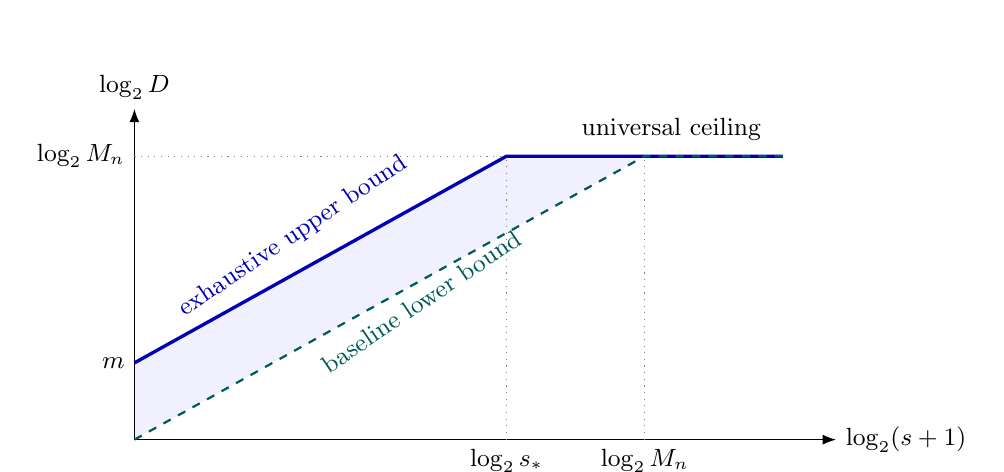
\begin{tikzpicture}[x=1.35cm,y=.75cm,>=Latex,font=\small]
 \fill[blue!6] (0,0)--(0,1.3)--(3.5,4.8)--(4.8,4.8)--cycle;
 \draw[->] (0,0)--(6.6,0) node[right] {$\log_2(s+1)$};
 \draw[->] (0,0)--(0,5.6) node[above] {$\log_2 D$};
 \draw[gray,dotted] (0,4.8)--(6.1,4.8);
 \draw[blue!70!black,very thick] (0,1.3)--(3.5,4.8)--(6.1,4.8);
 \draw[teal!70!black,thick,dashed] (0,0)--(4.8,4.8)--(6.1,4.8);
 \draw[gray,dotted] (3.5,0)--(3.5,4.8);
 \draw[gray,dotted] (4.8,0)--(4.8,4.8);
 \node[above,rotate=34,blue!70!black] at (1.6,3.15) {exhaustive upper bound};
 \node[below,rotate=34,teal!70!black] at (2.6,2.6) {baseline lower bound};
 \node[above] at (5.05,4.9) {universal ceiling};
 \node[below] at (3.5,0) {$\log_2 s_*$};
 \node[below] at (4.8,0) {$\log_2 M_n$};
 \node[left] at (0,1.3) {$m$};
 \node[left] at (0,4.8) {$\log_2 M_n$};
\end{tikzpicture}
\caption{Schematic baseline bounds, suppressing additive constants on
logarithmic axes. The shaded region represents a gap between bounds,
not proved amplification. The lower bound is proved in
Proposition~\ref{prop:baseline}. The structural bounds in
Sections~\ref{sec:sharing} and~\ref{sec:consistency-graph} can improve the upper curve.}
\label{fig:envelope}
\end{figure}

\paragraph{A ceiling is not a hardness theorem.}
Once $2^m s$ exceeds $M_n$, the upper bound flattens. This does
\emph{not} establish that $D(n,m,s)$ has reached $M_n$. Attainment is
immediate only for $s\ge M_n$, when a hardest function of $x$ itself
is an allowed verifier. Whether much smaller verifiers can project to
near-maximal functions is part of the question.

\paragraph{Verifiers near their own maximum.}
The relevant maximum for $f$ is $M_{n+m}$, not $M_n$. If
$\C(f)\ge\alpha2^{n+m}/(n+m)$ for a fixed $\alpha>0$, then
\begin{equation}\label{eq:maximum-ratio}
 \frac{\C(g)}{2^m\C(f)}
    =O\!\left(\frac{n+m}{\alpha n}\,2^{-2m}\right).
\end{equation}
For growing $m$ this is an enormous relative saving. It says nothing
by itself about whether $g$ has small absolute complexity.

\section{Circuit structure yields a second easy range}\label{sec:sharing}

\begin{lemma}[Effective inputs]\label{lem:inputs}
The output cone of a circuit with $s\ge1$ gates contains at most $s+1$
distinct input vertices. In particular, only that many witness inputs
can matter. A function depending essentially on $t$ inputs requires
at least $t-1$ gates.
\end{lemma}
\begin{proof}
Delete all vertices outside the output cone. If it contains $t$ input
vertices and $s$ gates, its underlying undirected graph is connected,
so it has at least $s+t-1$ wires. Fan-in at most two gives at most
$2s$ wires. Hence $t\le s+1$. Essential variables must occur in
every circuit for the function.
\end{proof}

For a chosen circuit, let $a$ and $b$ be its numbers of used ordinary
and witness inputs. Constants can be propagated, removing irrelevant
pins without increasing size in $B_2$. Apart from constant functions,
we can therefore take the output cone to have no constant vertices.
The case of an output that is a single input is immediate below.

\subsection{Sharing identical restrictions}

For a gate $v$, let $Y_v$ be the set of witness inputs in its syntactic
dependency cone, and write $k_v=|Y_v|$. Let $k$ be the corresponding
number at the output.

\begin{proposition}[A support-sensitive construction]\label{prop:support}
For a circuit with gates $V$ and a gate as output,
\begin{equation}\label{eq:support}
 \C(g)\le\sum_{v\in V}2^{k_v}+2^k-1.
\end{equation}
\end{proposition}
\begin{proof}
For each $v$ and each assignment $\alpha\in\B^{Y_v}$, create one
copy of $v$. Its inputs are the copies of its predecessors indexed by
the restrictions of $\alpha$ to their witness supports. Ordinary input
wires are shared; witness inputs are constants. Induction along the
circuit proves correctness. OR the $2^k$ output copies.
\end{proof}

In particular, the part of the verifier independent of $y$ need only
be computed once. This bound charges syntactic supports; simplifying
restricted gates can give further savings.

\subsection{Cutting shared witness inputs and gate outputs}

There is another construction that handles circuits close to trees.
Its proof is useful because it pinpoints the consistency that must be
retained when branches share witnesses. The underlying expansion of
copying constraints into consistent zero/one choices is established
in tensor-network counting
\citep[Theorem 17 of the author version]{BiamonteMortonTurner2015}.
Here we keep ordinary inputs symbolic and track the $B_2$ gate budget.

\begin{lemma}[Eliminating witnesses in a forest]\label{lem:forest}
Suppose a collection of formulas has $q$ gates in total, ordinary input
variables may repeat, and each witness variable occurs at most once
in the entire collection. The assertion that there is a witness
assignment making every formula output its prescribed bit has a
deterministic circuit of size $O(q+\ell+1)$, where $\ell$ is the
number of leaves and roots.
\end{lemma}
\begin{proof}
For each formula node $v$, compute two predicates $P_v^0(x),P_v^1(x)$:
which output values can its subtree realize by assigning its witnesses?
At an ordinary input $x_i$, the pair is $(\neg x_i,x_i)$; at a witness
leaf it is $(1,1)$; and at a constant $c$ it is $(1-c,c)$.
For a binary gate $v=h(u,w)$, use
\begin{equation}\label{eq:possible-values}
 P_v^c=\OR_{\substack{d,e\in\B\\h(d,e)=c}}
                    (P_u^d\land P_w^e).
\end{equation}
For a unary gate, use the analogous disjunction over its possible
input values.
The two subtrees have disjoint witness sets, so the indicated choices
can be realized simultaneously for each fixed $x$. Each gate costs
only a constant number of gates for its two predicates. Take the AND
of the appropriate predicates at the roots. Witness sets of different
trees are also disjoint. Repeated ordinary inputs cause no problem:
they keep the same fixed values throughout.
\end{proof}

\begin{theorem}[Simulation by fixing shared vertices]\label{thm:cut}
Consider a constant-free output cone with $s\ge1$ gates, $a$ ordinary
inputs, and $b$ witness inputs. Let $r$ count the witness-input and
gate vertices whose fan-out is at least two. Then
\begin{equation}\label{eq:cut}
 \C(g)=O((s+1)2^r),
 \qquad r\le s+1-a-b.
\end{equation}
Ordinary input vertices are not included in $r$.
\end{theorem}
\begin{proof}
Let $S$ be the set of the $r$ indicated vertices. Enumerate a bit
assignment $\beta\in\B^S$. Replace every \emph{use} of a vertex in
$S$ by its assigned bit. If that vertex is a gate, retain its defining
gate and impose the equation that its computed output equals its
assigned bit. Also require the original circuit output to be one.

After these cuts, every remaining gate output is used at most once,
and every unfixed witness input is used at most once. The defining
equations for the cut gates, together with the original output
condition, form a forest of formulas. It has $O(s+1)$ total gates,
leaves, and roots; ordinary inputs may repeat. Lemma~\ref{lem:forest}
gives an $O(s+1)$-gate circuit for this branch. OR the $2^r$ branches.

For correctness, a satisfying assignment of the original circuit
supplies a branch assignment by taking the actual values of the cut
vertices. Conversely, a satisfying branch supplies compatible
assignments to the remaining, disjoint witness sets. Restoring the cut
wires, the retained defining equations ensure by topological induction
that every assigned gate value equals its original computed value.
Thus the original output is one. The defining equations are essential;
guessing gate values without checking them would be unsound.

For the bound on $r$, let $E$ be the number of wires. Every vertex
except the output has fan-out at least one. Therefore
\[
 \sum_{v\ne\mathrm{out}}(\fanout(v)-1)
     =E-(s+a+b-1)\le s+1-a-b.
\]
Every counted vertex contributes at least one to this nonnegative sum.
\end{proof}

\begin{corollary}[A size-dependent universal bound]\label{cor:size-exponent}
Every verifier of complexity $s$ satisfies
\begin{equation}\label{eq:size-exponent}
 \boxed{\quad
 \C(g)=O\!\left((s+1)2^{\min\{m,n,(s+1)/3\}}\right).
 \quad}
\end{equation}
Consequently this estimate can be added to the minimum in
\eqref{eq:envelope}.
\end{corollary}
\begin{proof}
Normalize an optimal verifier circuit as above and let $s'\le s$
be its remaining size. For a nontrivial output cone put
$d=s'+1-a-b\ge0$. Exhaustive expansion costs $O((s'+1)2^b)$.
Truth-table synthesis on the $a$ used ordinary inputs costs
$O((s'+1)2^a)$, even by a minterm construction since $a\le s'+1$.
Theorem~\ref{thm:cut} costs $O((s'+1)2^d)$. Taking the minimum gives
\[
 \C(g)=O((s'+1)2^{\min\{a,b,d\}}).
\]
Since $a+b+d=s'+1$, this exponent is at most $(s'+1)/3$;
it is also at most $n$ and $m$. Constant and single-input outputs
obey the bound directly.
\end{proof}

For example, if a verifier depends on all $n+m$ inputs and has
$s=n+m-1+d$ gates, then $\C(g)=O((s+1)2^d)$. If $d=O(\log s)$,
the projection has polynomial-size circuits even when $m$ is large.
Without a full-input-dependence assumption, the unconditional
$2^{(s+1)/3}$ bound still saves an exponential factor over $2^m$
whenever $s+1\le(3-\delta)m$ for fixed $\delta>0$.

\begin{remark}[What the coefficient means]
The factor $1/3$ follows from balancing three quantities: used ordinary
inputs, used witness inputs, and the available excess fan-out. It is
an elementary upper bound, not an optimality claim or a known exact
transition. The argument is specific to gate count and fan-in two.
\end{remark}

\section{A stronger simulation from the consistency graph}
\label{sec:consistency-graph}

Fixing every shared vertex is sufficient, but it discards the arrangement
of those vertices. The graph may permit a sequence of small intermediate
tables even when the total number of shared values is large. We now use
that arrangement. The proof combines a circuit-specific count of consistency
constraints with a published theorem on pathwidth. Its quantitative
consequence improves the preceding $1/3$ exponential rate to $1/5$.

The basic operation is simple: keep a table of which assignments to the
current boundary can be extended through the processed part. Each table
entry is a circuit on $x$. Ordinary inputs remain shared circuit wires;
they are never enumerated as table indices.

\subsection{Separate ordinary computation from consistency}

Normalize and prune the supplied circuit. If its output has no syntactic
witness dependency, its existing circuit computes the projection. If its
output is a witness input, the projection is one. Otherwise partition the
gates into $p$ gates independent of the witnesses and $q\ge1$ dependent
gates. Compute the independent gates once. Let
$h_1(x),\ldots,h_h(x)$ be the distinct independent signals entering
dependent gates, including direct ordinary inputs, and let $b$ be the
number of used witnesses. Let $\ell$ count input pins of dependent
gates supplied by a witness or a dependent gate. Then
\begin{equation}\label{eq:core-pins}
 \ell+h\le2q.
\end{equation}
Here $h$ counts distinct signals, while $\ell$ counts pins, with
multiplicity. Every dependent gate has at least one dependent input,
so it has at most one independent input.

Introduce a consistency variable for every witness and every dependent
gate output. A gate $v$ contributes the constraint
\[
 A_v=[z_v=\operatorname{op}_v(\text{predecessor values})],
\]
and the output contributes $[z_{\mathrm{out}}=1]$. The ordinary
signals in these expressions remain functions of $x$. Form a bipartite
incidence graph $H$ with one vertex for each consistency variable and
each constraint, and one edge for each incidence. Retain multiple
incidences if a value supplies two pins.

\begin{lemma}[The consistency budget]\label{lem:consistency-budget}
The graph $H$ is connected and has
\[
 |V(H)|=2q+b+1,\qquad |E(H)|=q+\ell+1.
\]
Its cycle rank $\kappa=|E(H)|-|V(H)|+1$ therefore satisfies
\begin{equation}\label{eq:consistency-budget}
 \boxed{\quad \kappa=\ell-q-b+1,\qquad h+b+\kappa\le q+1.\quad}
\end{equation}
If the full cone has $s=p+q$ gates and $a$ used ordinary inputs, then
also $\kappa\le s+1-a-b$.
\end{lemma}
\begin{proof}
Every dependent gate and used witness has a directed path through
dependent gates to the output. The incidence graph subdivides those
connections and adds the output constraint, proving connectivity and
the counts. Equation~\eqref{eq:core-pins} gives the boxed inequality.
For the last assertion, delete the ordinary inputs and independent
gates from the full cone's underlying undirected multigraph. The
remaining graph has $q+b$ vertices and $\ell$ edges, and hence cycle
rank $\kappa$. Deletion cannot increase cycle rank, as follows by
restricting the binary cycle space. The full cone has at most $2s$
edges and $s+a+b$ vertices, giving the claimed bound.
\end{proof}

The conjunction of the constraints, quantified over all consistency
variables, equals $g$. An original witness assignment extends uniquely
to its gate values. Conversely, the equations force those values by
topological induction. This observation preserves the consistency that
naive separate existential evaluation loses.

\subsection{Small tables reduce the graph to a cubic graph}

Give every incidence edge its own binary index. At a variable vertex,
place the equality table: its entry is one exactly when all incident
indices agree. At a constraint vertex, place the constraint's truth
table on its incident indices. A degree-one equality table has both
entries one. A gate table has at most three indices. After fixing its
indices, its entry is a constant, some $h_i(x)$, or its complement.
Thus the $p$ independent gates and at most $h$ additional complements
prepare every table entry.

We call these arrays \emph{Boolean tensors}; no numerical approximation
is involved. Contracting an edge means ORing over its binary value and
ANDing the two incident entries. Distributivity proves that contraction
preserves the represented function, pointwise for each fixed $x$.

\begin{lemma}[A cubic reduction with linear circuit cost]
\label{lem:cubic-reduction}
The consistency tables reduce, using $O(q+1)$ extra gates, to a scalar
factor and either an empty graph or a simple connected cubic graph
$K$. If $N=|V(K)|>0$, then
\[
 N=2(\kappa(K)-1)\le2(\kappa-1).
\]
Every surviving table still has at most eight entries, each represented
by an already constructed circuit wire.
\end{lemma}
\begin{proof}
First replace each equality vertex of degree $D\ge4$ by a tree of
$D-2$ ternary equality vertices. The internal edge values are uniquely
determined when the external values agree. This adds $D-3$ vertices
and edges, preserving cycle rank and connectivity. The new equality
vertex count is at most the sum $q+\ell+1$ of the old variable degrees.
Including constraint vertices, the resulting subcubic graph has
\[
 N_0\le q+1+(q+\ell+1)\le4q+2
\]
vertices. A loop counts twice toward degree.

Apply the following exact table operations until none applies.
\begin{enumerate}
 \item Remove a rank-zero table and AND its scalar into an accumulator.
 \item For a loop, identify its two ports and OR the two diagonal
 entries. There are at most two remaining entries. Summing all four
 combinations would violate the equality of the loop's two ends.
 \item At a loop-free vertex of degree one or two, contract one edge
 into its neighbor. The resulting rank is at most three. Each of at
 most eight entries needs two ANDs and one OR, costing at most 24 gates.
 Any second edge between the same vertices becomes a loop.
 \item If two cubic vertices share two edges, contract both at once.
 The four resulting entries each use four ANDs and three ORs, costing
 28 gates. Three parallel edges instead produce one scalar using at
 most 15 gates.
\end{enumerate}
Each operation decreases $|V|+|E|$, costs at most 32 gates, and keeps
degree at most three. Initially $|E|\le3N_0/2$, so 80$N_0$ gates
suffice for all reductions, including the scalar accumulator.

Contracting an ordinary edge preserves cycle rank; removing a loop
lowers it by one; contracting $j$ parallel edges lowers it by $j-1$.
The remaining nonempty graph stays connected. At termination it is
simple and every degree is three. Hence $|E(K)|=3N/2$, and its cycle
rank is $N/2+1$. This proves the assertion.
\end{proof}

The treatment of loops and parallel edges matters. Silently deleting
them as graph-theoretic nuisances would change the represented function.
The reductions above manipulate their actual tables at a charged cost.

\subsection{From a path decomposition to a circuit}

A \emph{path decomposition} is a sequence of bags containing all
vertices, containing both ends of every edge in some bag, and containing
each vertex in a consecutive interval of bags. Its width is the largest
bag size minus one; pathwidth is the minimum such width. The cutwidth
of a vertex ordering is the largest number of edges crossing between
a prefix and the remaining vertices.

\begin{lemma}[A width conversion for cubic graphs]\label{lem:median-width}
A simple cubic graph of pathwidth $k$ has a vertex ordering of cutwidth
at most $k+2$.
\end{lemma}
\begin{proof}
Given bags $B_1,\ldots,B_L$, represent $v$ by
$I_v=[\operatorname{first}(v)-1/4,\operatorname{last}(v)+1/4]$.
At most $k+1$ intervals contain any point. For each edge $e=uv$ choose
a distinct timestamp $t_e$ in the interior of $I_u\cap I_v$, which
is nonempty. Place $v$ at the median $t_v$ of its three incident
timestamps and order the vertices by these medians.

Consider a cut at a point $t$ distinct from all timestamps. For a
crossing edge with $t_u<t<t_v$, charge it to $u$ if $t_e>t$, and to
$v$ otherwise. The charged interval contains $t$. A vertex receives
at most one charge: it has just one incident timestamp strictly above
its median and just one strictly below it. Thus there are at most
$k+1$ crossing edges.

At a cut between tied medians, at most two vertices are tied, because
the edge timestamps are distinct and an edge has two endpoints. Apply
the same charging rule to every other crossing edge. Only the edge
whose timestamp equals the common median can remain uncharged, adding
at most one. This proves the $k+2$ bound and gives an explicit ordering.
\end{proof}

This width conversion is consistent with established graph-search
relations; it is included with a proof to make the numerical exponent
checkable. Section~\ref{sec:prior-work} records the attribution.

\begin{lemma}[Symbolic frontier contraction]\label{lem:frontier}
Given an ordering of $K$ of cutwidth $w$, its tensor value has a circuit
using fewer than $4N2^w$ additional gates.
\end{lemma}
\begin{proof}
Let $F_i$ be the edges leaving the first $i$ vertices. For each
$\alpha\in\B^{F_i}$ maintain a wire $P_i(\alpha;x)$: the OR over
internal edge assignments of the AND of all processed table entries,
with the boundary fixed to $\alpha$. Start with $P_0=1$.

At the next vertex let $J$ be its $j$ edges into the processed prefix.
For each new boundary assignment, OR over the $2^j$ assignments to
$J$ the AND of the appropriate old entry and local table entry. This
preserves the stated meaning by distributivity. Its gate cost is
\[
 2^{|F_i|}(2^{j+1}-1)<2^{|F_i|+j+1}.
\]
Because $|F_i|=|F_{i-1}|+3-2j$ and both frontier sizes are at most
$w$, one has $|F_i|+j\le w+1$: use the new frontier for $j=0,1$
and the old frontier for $j=2,3$. Each vertex therefore costs less
than $2^{w+2}$ gates. At the last vertex there are no boundary indices
and the single entry is the desired scalar.
\end{proof}

The complete finite construction costs at most
\begin{equation}\label{eq:finite-tensor-cost}
 p+h+80N_0+4N2^w+1\le p+400(q+1)2^w.
\end{equation}
For an empty reduced graph the frontier construction is unnecessary;
take $N=w=0$ and use the scalar accumulator. Ordinary computation is
paid once, including when its result appears in many boundary entries.

\subsection{The improved exponential rate}

We use the following published graph theorem: for every $\eta>0$
there is $n_\eta$ such that every simple subcubic graph on $N>n_\eta$
vertices has pathwidth at most $(1/6+\eta)N$. A suitable decomposition
can be constructed in polynomial time for fixed $\eta$
\citep[Theorem 5 and Section 4]{FominHoie2006}.

\begin{theorem}[Projection controlled by consistency cycles]
\label{thm:cycle-simulation}
For every $\delta>0$ there is a constant $A_\delta$ such that
\begin{equation}\label{eq:cycle-simulation}
 \C(g)\le p+A_\delta(q+1)2^{(1/3+\delta)\kappa}.
\end{equation}
For example, $A_\delta=400\cdot2^{n_{\delta/2}+2}$ suffices using
the threshold in the cited theorem. No uniform small value of this
constant, or endpoint bound $O((q+1)2^{\kappa/3})$, is asserted.
\end{theorem}
\begin{proof}
Use the cubic reduction and the graph theorem with $\eta=\delta/2$.
Since $N\le2\kappa$, Lemma~\ref{lem:median-width} gives
$w\le(1/3+\delta)\kappa+2$ for large $N$. The finitely many smaller
graphs are covered by adding $n_{\delta/2}$ to the exponent. Apply
\eqref{eq:finite-tensor-cost}.
\end{proof}

\begin{theorem}[A universal $1/5$ exponential rate]\label{thm:fifth}
Set $\alpha=1/3+\delta$ and $\beta=\alpha/(1+2\alpha)$.
With the preceding notation,
\begin{equation}\label{eq:core-fifth}
 \C(g)\le p+O_\delta\!\left((q+1)
                    2^{\min\{h,b,\alpha\kappa\}}\right)
 \le p+O_\delta\!\left((q+1)2^{\beta(q+1)}\right).
\end{equation}
In particular, for every $\varepsilon>0$,
\begin{equation}\label{eq:fifth}
 \boxed{\quad
 D(n,m,s)=O_\varepsilon\!\left(
  \min\left\{\frac{2^n}{n},\ (s+1)2^m,
       (s+1)2^{(1/5+\varepsilon)(s+1)}\right\}\right).
 \quad}
\end{equation}
The comparison with $2^n/n$ assumes $n\ge2$ as before.
\end{theorem}
\begin{proof}
Two alternatives to \eqref{eq:cycle-simulation} are
$p+O((q+1)2^b)$ by witness enumeration and $p+M_h$ by treating
the $h$ independent signals as formal input bits. Substituting their
actual values after synthesis is valid even when those values are
correlated. The bound $M_h=O(2^h)$, also valid for $h=0,1$, suffices.
Take the minimum of these three estimates. If
$z=\min\{h,b,\alpha\kappa\}$, the consistency budget gives
\[
 (2+1/\alpha)z\le h+b+\kappa\le q+1.
\]
This proves \eqref{eq:core-fifth}. Since $\beta\to1/5$ as
$\delta\downarrow0$, and $p+q\le s$ after normalization, the
claimed universal bound follows. Trivial outputs were handled before
the construction.
\end{proof}

This is a circuit-size theorem. In particular, the synthesis of an
arbitrary function on the formal inputs does not promise that its
truth table can be discovered in the size of the resulting circuit.
The numerical rate comes from three precise facts: $h+b+\kappa\le q+1$,
at most $2\kappa$ vertices in the cubic reduction, and pathwidth at
most $N/6+o(N)$. It is not a claim that the coefficient $1/5$ is optimal.

\begin{figure}[ht]
\centering
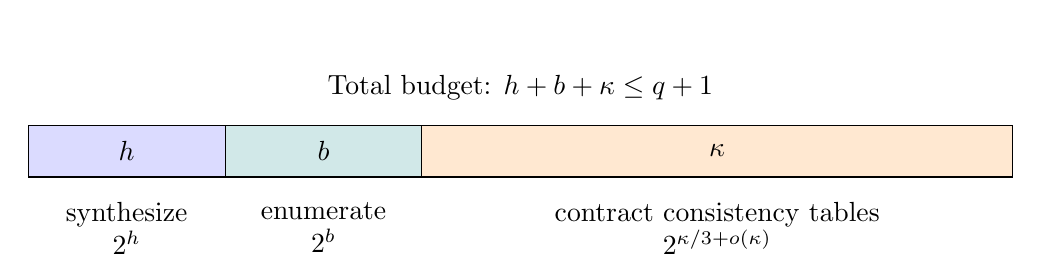
\begin{tikzpicture}[x=1.25cm,y=1cm]
 \fill[blue!14] (0,0) rectangle (2,0.65);
 \fill[teal!18] (2,0) rectangle (4,0.65);
 \fill[orange!18] (4,0) rectangle (10,0.65);
 \draw (0,0) rectangle (10,0.65);
 \draw (2,0)--(2,0.65) (4,0)--(4,0.65);
 \node at (1,0.33) {$h$};
 \node at (3,0.33) {$b$};
 \node at (7,0.33) {$\kappa$};
 \node[anchor=south] at (5,0.85) {Total budget: $h+b+\kappa\le q+1$};
 \node[align=center,anchor=north] at (1,-0.2)
   {synthesize\\$2^h$};
 \node[align=center,anchor=north] at (3,-0.2)
   {enumerate\\$2^b$};
 \node[align=center,anchor=north] at (7,-0.2)
   {contract consistency tables\\$2^{\kappa/3+o(\kappa)}$};
\end{tikzpicture}
\caption{The limiting balance is $h:b:\kappa=1:1:3$.
All three exponents then approach $(q+1)/5$.
This balances upper bounds; it supplies neither a hard example nor
a proof that this rate is optimal. Ordinary preprocessing costs $p$
additional gates, once.}
\label{fig:consistency-budget}
\end{figure}

\paragraph{Why the independent part should stay outside the exponent.}
For $t\ge3$, put $a_i=x_{2i-1}\land x_{2i}$ and
\[
 H_t(x)=\bigoplus_{1\le i<j\le t}(a_i\land a_j),
 \qquad f_t(x,y)=H_t(x)\land(y_1\lor\cdots\lor y_t).
\]
Compute all $a_i$, their pair products, an XOR chain, the witness OR
chain, and the final AND. This supplied circuit has
$p=t^2-1$, $q=b=t$, $h=1$, and $\kappa=0$.
The projection is $H_t$, with a circuit of size $p$.
Every ordinary input is essential: set one other $a_j$ to one,
all remaining pairs to zero, and the other bit of the chosen pair to
one. Every witness is essential when $H_t=1$ and the other witnesses
are zero. Thus unused inputs do not explain the simplification.

The full undirected circuit graph contains a subdivision of $K_t$,
with the $a_i$ as branch vertices and their pair-product gates on
the edges. Its treewidth is at least $t-1$, although the consistency
graph is a tree. Also $r=t$ for the old shared-vertex bound, whereas
the new structural bound is $O(t^2)$. Coverage independently detects
a one-witness cover in this example. The example explains a distinction
between structural parameters, not a circuit lower bound or an example
attaining the $1/5$ exponent.

\subsection{Condition a few values before eliminating the rest}

\begin{corollary}[Conditioning and componentwise elimination]
\label{cor:condition-cycles}
Fix $t$ consistency variables in every possible way, retaining all
defining equations. Let $\kappa_*$ be the largest cycle rank of a
connected component of the remaining incidence graph. Then
\[
 \C(g)\le p+O_\delta\!\left((q+1)
                  2^{t+(1/3+\delta)\kappa_*}\right).
\]
\end{corollary}
\begin{proof}
In each branch, distinct components have disjoint quantified variables.
Their projections may therefore be ANDed for each fixed $x$. Apply the
construction to each component; their total size is $O(q+1)$ and their
individual exponents are bounded by $(1/3+\delta)\kappa_*$. OR the
$2^t$ branches. The independent signals remain shared. Consistency
equations make the conditioning sound, exactly as in Theorem~\ref{thm:cut}.
\end{proof}

Conditioning combined with elimination is an established algorithmic
architecture. Here it supplies a refinement of the explicit circuit
bound, useful when a small set of shared values separates otherwise
difficult parts. The relevant exponent uses the largest residual
component, rather than the sum of its components' cycle ranks.

\subsection{The uniform SAT and exact-counting algorithm}
\label{sec:counting-algorithm}

We now prove the algorithmic guarantee highlighted in
Section~\ref{sec:algorithm-overview}. The nonuniform theorem used
synthesis on formal ordinary inputs.
The all-quantified case has no such step. Its explicit table operations
also preserve counts, which gives the following algorithmic consequence.
This statement includes its proof; the unresolved issue in
Section~\ref{sec:prior-work} is comparison and priority.

\begin{corollary}[Counting by the gate-minus-input budget]
\label{cor:gate-counting}
Fix $\delta>0$ and write $\alpha=1/3+\delta$. Given a single-output
$B_2$ circuit with $s$ gates and $u$ input bits, one can count its
satisfying inputs in time
\[
 \poly_\delta(s+u+1)\,
 2^{\min\{b,\alpha(s+1-b)\}},
\]
where $b$ is the number of inputs remaining in a normalized output
cone. In particular, for every fixed $\varepsilon>0$, the time is
\[
 \poly_\varepsilon(s+u+1)\,
 2^{(1/4+\varepsilon)(s+1)}.
\]
The space used is at most polynomial times the same exponential
factor. A polynomial-space bound is not asserted.
\end{corollary}
\begin{proof}
Prune the output cone and propagate constants and unary redundancies
without changing the function. Inputs removed from the cone are free;
their contribution is a final multiplicative factor $2^{u-b}$.
Constant and designated-input outputs are evaluated directly. For the
remaining circuit quantify all $b$ inputs, so there are no independent
signals. Its consistency rank satisfies $\kappa\le s+1-b$.

Replace Boolean OR and AND in the tensor construction by integer
addition and multiplication. The original tables contain only zeros
and ones. For each satisfying input, the circuit equations specify
exactly one gate-value assignment. Incidence equality tables specify
exactly one set of equal edge values, and their ternary expansions have
exactly one internal extension. Thus the initial tensor contraction
counts satisfying inputs, with no spurious multiplicity.

Every reduction in Lemma~\ref{lem:cubic-reduction} is a distributive
identity, including diagonal loop sums and joint parallel-edge sums.
It remains valid over the nonnegative integers. More explicitly, a
reduced table entry is the number of internal edge assignments in its
contracted region that satisfy the original tables, conditional on its
boundary. A contraction combines disjoint regions and sums over their
shared indices, preserving this interpretation. The same invariant
holds for the frontier entries in Lemma~\ref{lem:frontier}.

There are $O(s+1)$ indices after equality expansion. Each table entry
is therefore bounded by $2^{O(s+1)}$, so its bit length is $O(s+1)$.
Integer additions and multiplications have polynomial bit cost; the
last factor $2^{u-b}$ only shifts the answer. For fixed $\delta$, the
cited constructive pathwidth theorem and median conversion find the
required order in polynomial time. The bounded-size graphs below its
threshold are handled by exhaustive order search, a constant depending
on $\delta$. The operation count is consequently polynomial times
$2^{\alpha(s+1-b)}$, with exponential-size frontiers allowed.

Alternatively enumerate the $2^b$ used-input assignments, evaluate the
circuit, and count the accepting ones. Choose the cheaper proved bound.
Finally,
\[
 \min\{b,\alpha(s+1-b)\}
 \le\frac{\alpha}{1+\alpha}(s+1),
 \qquad \frac{\alpha}{1+\alpha}\longrightarrow\frac14.
\]
This proves both time estimates and the stated space majorant.
\end{proof}

Testing whether the count is nonzero decides circuit satisfiability.
For any fixed $0<\gamma<4$, the bound also gives a running time
$2^{(1-\Omega_\gamma(1))u}\poly(u)$ when
$s\le(4-\gamma)u$, after choosing a sufficiently small fixed
$\varepsilon$. This consequence uses exponential space and the exact
$B_2$ gate convention. Its numerical comparison with previously
reported circuit-SAT algorithms deserves particular scrutiny.

\subsection{What critical amplification would force}
\label{sec:critical-balance}

The coefficient $1/5$ comes from balancing three upper bounds.
Near equality therefore forces several structural conditions
simultaneously. The following statements concern a normalized circuit
with $q\ge1$ and a witness-dependent gate as output, using the notation
of Section~\ref{sec:consistency-graph}.

\begin{lemma}[Finite stability of the three-way balance]
\label{lem:finite-stability}
Fix $\delta>0$, put $\alpha=1/3+\delta$, and choose $A_\delta\ge1$
large enough for
\[
 \C(g)\le p+A_\delta(q+1)2^{\min\{h,b,\alpha\kappa\}}.
\]
If $t\ge0$ and $\C(g)\ge p+A_\delta(q+1)2^t$, then
\[
 \Delta=q+1-(2+1/\alpha)t\ge0,
\]
and there are $e_h,e_b,e_\kappa\ge0$ satisfying
\[
 h=t+e_h,\qquad b=t+e_b,\qquad
 \kappa=t/\alpha+e_\kappa,\qquad
 e_h+e_b+e_\kappa\le\Delta.
\]
\end{lemma}
\begin{proof}
Comparing the two size inequalities forces
$h,b,\alpha\kappa\ge t$. Subtract these lower bounds from
$h+b+\kappa\le q+1$.
\end{proof}

This elementary lemma is useful because it preserves the fixed-$\delta$
constant before any limit is taken. Its asymptotic consequence also
constrains the residual graph, beyond the original cycle count.

\begin{theorem}[Necessary structure at the critical gate budget]
\label{thm:critical-structure}
Consider a family with $m\to\infty$ declared witness bits, normalized
size $s=p+q$, and
\[
 s+1=(5+o(1))m,\qquad \log\C(g)\ge m-o(m).
\]
Let $a$ be the number of used ordinary inputs. Then
\begin{align*}
 p&=o(m),& q&=(5+o(1))m,\\
 a,h,b&=(1+o(1))m,& \kappa&=(3+o(1))m.
\end{align*}
For every choice of legal equality splitting and reductions in
Lemma~\ref{lem:cubic-reduction}, the resulting kernel $K$ is
eventually nonempty and satisfies
\begin{align*}
 |V(K)|&=(6+o(1))m,& \kappa-\kappa(K)&=o(m),\\
 \operatorname{cw}(K)&=(1+o(1))m,&
 \operatorname{pw}(K)&=(1+o(1))m.
\end{align*}
Here cutwidth and pathwidth mean their minimum over all orders and
decompositions. No hard family satisfying the hypotheses is asserted.
\end{theorem}
\begin{proof}
Since $p=O(m)$ whereas $\C(g)\ge2^{m-o(m)}$,
$\log(\C(g)-p)\ge m-o(m)$. For each fixed $\delta>0$,
Theorem~\ref{thm:fifth} therefore gives
\[
 h\ge m-o(m),\qquad b\ge m-o(m),\qquad
 \kappa\ge m/\alpha-o(m).
\]
The prefactor contributes only $O_\delta(\log m)$ to the logarithm.
Using $p+h+b+\kappa\le s+1$, we obtain
\[
 \limsup \frac{p}{m}\le3-1/\alpha,\qquad
 \limsup \frac{h}{m},\ \limsup\frac{b}{m}\le4-1/\alpha.
\]
These inequalities hold for every fixed $\delta$. Letting $\delta$
tend to zero after taking the limits proves $p=o(m)$ and
$h/m,b/m\to1$. The budget and the fixed-$\delta$ lower bounds
then give $\kappa/m\to3$, and $q/m\to5$ follows from $s=p+q$.

To relate $a$ to $h$, note first that $h\le a+p$. In the undirected
graph on the $a$ ordinary inputs and $p$ independent gates, every
connected component contains an interface signal, because every
vertex is in the output cone. If there are $c$ components, then
$c\le h$, and counting edges gives
$a+p-c\le2p$. Thus $a\le p+h$, so $|a-h|\le p$ and $a/m\to1$.

Fix any sequence of legal reductions along the family. An empty
kernel would give $\C(g)=O(s)$, so eventually it is nonempty.
Write $N=|V(K)|$. The finite compiler bound, applied to an order
of minimum cutwidth, gives
\[
 \C(g)\le p+400(q+1)2^{\operatorname{cw}(K)},
 \qquad \operatorname{cw}(K)\ge m-o(m).
\]
The cutwidth lower bound and $\operatorname{cw}(K)\le3N/2$ imply
$N\to\infty$. On the other hand $N\le2(\kappa-1)\le6m+o(m)$. For every fixed
$\eta>0$, the cubic pathwidth theorem and
Lemma~\ref{lem:median-width} give, for sufficiently large $N$,
\[
 \operatorname{cw}(K)\le\operatorname{pw}(K)+2
       \le(1/6+\eta)N+2.
\]
Hence $\liminf N/m\ge1/(1/6+\eta)$ for every $\eta>0$, proving
$N/m\to6$. The cubic identity $\kappa(K)=N/2+1$ gives the cycle
loss. The same inequalities sandwich each width between $m-o(m)$
and $m+o(m)$. All constants depend only on the fixed slack, so this
argument applies to any selected legal reduction sequence.
\end{proof}

There is little unused fanin capacity in such a family. If $r$ counts
independent-signal input pins of the dependent gates, with multiplicity,
and $U=2q-(\ell+r)$, then
\[
 q+1-h-b-\kappa=U+(r-h)=o(m).
\]
Both terms are nonnegative. Thus only $o(m)$ input slots are missing
from binary gates, and ordinary signals have only $o(m)$ repeated
uses at the interface. This concerns distinct signals, not semantic
independence of their values.

\paragraph{Combining the structural and witness conditions.}
The hypotheses hold whenever $s+1=(5+o(1))m$ and
$\C(g)\ge T=2^m(s+1)/L$ with $\log L=o(m)$.
Corollary~\ref{cor:sparse-population} then also forces
$\Omega((T/n)\log(2+T/n))$ positive ordinary inputs with $O(nL)$
declared witnesses. Removing the $m-b$ unused witness bits divides
each positive fiber and this threshold by exactly $2^{m-b}$;
the two witness conventions must be kept consistent.
Enumeration already gives $m-b\le\log L$ under this amplification
hypothesis. These are simultaneous necessary conditions. Large
width, balanced budgets, and sparse fibers alone do not establish
a lower bound on $\C(g)$.

\subsection{Critical graph budgets can coexist with an easy projection}
\label{sec:kernel-realization}

The critical gate and cycle budgets alone do not force a hard
projection. A large class of cubic graphs can occur as exact residual
kernels with nearly critical budgets and a simple projection. The
distinction between the supplied circuit and a minimum circuit is
essential here.

\begin{theorem}[Cubic realization with controlled budgets]
\label{thm:kernel-realization}
Let $K$ be a finite simple 2-vertex-connected cubic graph and put
$k=|V(K)|/2+1$. Set $t=\lfloor k/3\rfloor+1$; when $K$ is
triangle-free, one may instead take $t=\lceil k/3\rceil$.
There is an acyclic AND-only verifier on $t$ ordinary and $t$ witness
inputs with
\[
 (p,q,h,b,\ell,\kappa)
   =(0,k+2t-1,t,t,2k+3t-2,k).
\]
It has no constants, unary gates, repeated input wires at a gate,
unused inputs, or gates outside its output cone. A specified legal
equality splitting and reduction sequence produces exactly $K$, with
zero cycle-rank loss. Every input is essential, but
\[
 f(x,y)=\AND_{i=1}^{t}x_i\land\AND_{j=1}^{t}y_j,
 \qquad g(x)=\AND_{i=1}^{t}x_i,
 \qquad \C(f)=2t-1,\quad \C(g)=t-1.
\]
Thus $h+b+\kappa=q+1$ and $t=k/3+O(1)$, while the supplied
circuit exceeds its minimum size by exactly $k$ gates.
\end{theorem}

The syntactic conditions in the statement are those used by the
compiler's normalization. They do not prohibit identities involving
several gates, such as associativity and idempotence of AND.
We give the construction and its accounting in full.

\begin{proof}
First give $K$ an acyclic orientation with one source and one sink.
This is the classical $st$-numbering property of 2-connected graphs
\citep{EvenTarjan1976}. An existence proof suffices here. Start with
a cycle, choose adjacent vertices $s,z$, and order the vertices along
the $s$-to-$z$ path obtained by deleting the edge $sz$. If some
vertices remain outside the current set, one of their components has
two distinct attachments to the current set; otherwise its unique
attachment would be a cut vertex. Choose a path through that component
between two such attachments $u,v$, with internal vertices outside.
Orient the path from its earlier to its later endpoint and insert its
internal vertices, in order, immediately after the earlier endpoint.
Every old internal vertex retains neighbors on both sides, and each
new vertex has its two path neighbors on opposite sides. Repeat until
all vertices are ordered and orient every edge forward. Only $s$ is
a source and only $z$ is a sink.

\emph{The circuit skeleton.}
Every other vertex is a fork with indegree one and outdegree two,
or a join with indegree two and outdegree one. If their numbers are
$F,J$, the degree sum gives
\[
 3+F=J+3,\qquad F+J+2=2(k-1),\qquad F=J=k-2.
\]
Put witness $y_1$ at $s$. A fork copies its incoming wire at no gate
cost. A join ANDs its incoming wires. At $z$, two AND gates combine
the three incoming wires. This skeleton has $k$ gates.
Temporarily assign each join output its own formal wire name, even
if that join receives the same name twice. Call such a join a conflict.

The sink receives at least two different names. Indeed a topologically
last join exists, and any path from it to the sink contains only forks.
If its output passes through a nonempty fork tree, a last fork would
have both outgoing edges to the sink, contradicting simplicity.
Its output therefore reaches the sink directly and on just one edge.
It cannot name all three sink inputs. Choose two distinct names for
the first sink gate; its new output and the third original input
are distinct at the second gate.

\emph{The conflict budget.}
The subgraph on the source and forks is a forest. A cycle with an
acyclic orientation would have a vertex with two incoming edges,
which these vertices cannot have. Its components are exactly the
trees carrying one formal wire name. A component not containing $s$
with $u$ forks has one incoming edge and $u+1$ outgoing edges. Each
conflict it supplies uses two outgoing edges. For $u=1$ there is no
conflict, by simplicity; for $u\ge2$ their number is at most
\[
 \left\lfloor\frac{u+1}{2}\right\rfloor\le\frac{2u}{3}.
\]
The inequality is checked directly at $u=2$ and follows from
$(u+1)/2\le2u/3$ for $u\ge3$.

The source component with $u$ additional forks has $u+3$ outgoing
edges. At $u=0$ it has no conflict; at $u=1,2$ it has at most two.
For $u\ge3$ its number of conflicts is at most
$\lfloor(u+3)/2\rfloor\le2u/3+4/3$.
The latter bound covers the small cases as well. Summing over all
$F=k-2$ forks bounds the total number $R$ of conflicts by
\[
 R\le\lfloor2k/3\rfloor.
\]
If $K$ is triangle-free, the $u=1$ source component has no conflict,
since one would make a triangle through the source, fork, and target
join. The source bound improves to $2u/3+1$, giving
\[
 R\le\lfloor(2k-1)/3\rfloor
 \qquad\text{in the triangle-free case}.
\]

There are $2t-1$ unused inputs available: the $t$ ordinary inputs and
$t-1$ additional witnesses. The chosen $t$ ensures $R\le2t-1$ in
each case. On one incoming edge of each conflicting join insert
\[
 \text{new wire}=\text{old wire}\land\text{fresh input},
\]
using a different input each time. Insert any remaining inputs by
such gates in a chain on one original edge. The fresh output names
split copied wires; they never identify distinct old names. Hence
all conflicts are repaired without creating new ones, including at
the two sink gates. The orientation gives a topological gate order.

\emph{The verifier budget and its function.}
Each attachment has a witness-dependent old input, so all gates are
witness-dependent. There are $k+2t-1$ gates, every ordinary input
appears at one gate pin, and all $t$ witnesses are used. Therefore
$p=0$, $h=b=t$, and
\[
 \ell=2q-t=2k+3t-2,\qquad
 \kappa=\ell-q-b+1=k.
\]
Every vertex reaches the unique sink. ANDing along the circuit thus
gives the conjunction of all inputs, proving the displayed $f,g$.
Each input is essential by setting all other inputs to one. The
effective-input lower bound in Lemma~\ref{lem:inputs},
met by an AND chain, gives $\C(f)=2t-1$ and $\C(g)=t-1$.

\emph{The exact residual kernel.}
Form the actual consistency incidence graph. A wire with $u$ forks
after its defining join has $u+1$ uses and one defining incidence.
Choose its equality splitting to be precisely that fork tree: an
equality of degree $u+2$ is replaced by $u$ ternary equalities.
For $u=0$, keep its degree-two equality. The source wire with $u$
forks has $u+3$ uses; choose its splitting into the source and those
$u$ forks. Attachments divide these trees into smaller pieces, to
which the same construction applies. Reversing these splittings
contracts each equality tree to the actual incidences of one circuit
wire, verifying that they are permitted choices in
Lemma~\ref{lem:cubic-reduction}.

Contract the output-one assertion through the output equality into
the second sink gate. That constraint now has two ports. Contract
the degree-two equality between the sink gates and then the remaining
two-port constraint into the first sink gate. Its surviving table
is the conjunction of the three original incoming bits, at vertex $z$.
For each additional witness, contract its degree-one equality into
its attachment constraint, leaving two ports. For example,
$\OR_y[v=u\land y]=[v\le u]$: the resulting table is retained,
not replaced by an equality. Ordinary attachments
already have two ports, since their ordinary inputs are coefficients.
Contract these two-port constraints and all degree-two wire equalities
along their original edges. Their updated neighboring tables retain
the semantic effects of the attachments.

Topologically these operations undo edge subdivisions, the sink tree,
and attached leaf trees. They leave exactly the marked vertices and
edges of $K$. No loop or parallel-edge reduction is needed: every
step is a permitted single-edge contraction and preserves cycle rank.
Since $K$ is simple and cubic, the reduction terminates there, with
the stated zero loss and the linear operation cost of the compiler.
\end{proof}

For triangle-free $K$ with $k=3t$, the parameters are exactly
\[
 (p,q,h,b,\ell,\kappa)=(0,5t-1,t,t,9t-2,3t).
\]
Thus acyclicity, essential inputs, the critical budget, and zero cycle
loss do not prevent these kernel topologies. The theorem asserts
existence of the specified reduction, not that every reduction must
return $K$. It does not realize the hardness hypothesis of
Theorem~\ref{thm:critical-structure}: its supplied circuit is
nonminimal and its projection is easy. Stronger semantic reductions
or choosing a smaller equivalent verifier can remove the apparent
structural difficulty.



\section{Many witnesses give small nonuniform circuits}

For $x$ with $g(x)=1$, define its witness set
$W_x=\{y:f(x,y)=1\}$. The minimum size of a set
$H\subseteq\B^m$ intersecting every nonempty $W_x$ is a natural
coverage parameter, say $\tau(f)$. For $g\equiv0$, take $\tau(f)=0$.
By evaluating only witnesses in $H$,
\begin{equation}\label{eq:cover}
 \C(g)\le\tau(f)s+\max\{\tau(f)-1,0\}.
\end{equation}

\begin{proposition}[Witness-density bound]\label{prop:density}
Suppose $n\ge1$ and every nonempty $W_x$ has size at least $K$, and set
$\rho=K/2^m>0$. There is a fixed set of at most
\begin{equation}\label{eq:hitting-size}
 T=\min\left\{2^m,
       \left\lceil\frac{n\ln2+1}{\rho}\right\rceil\right\}
\end{equation}
witnesses meeting all nonempty $W_x$. Hence
\begin{equation}\label{eq:density}
 \C(g)\le T(s+1)-1
       =O\!\left((s+1)\min\{2^m,n2^m/K\}\right).
\end{equation}
For the identically zero function, the conclusion holds trivially.
\end{proposition}
\begin{proof}
Take $t=\lceil(n\ln2+1)/\rho\rceil$ independent uniform witnesses.
A fixed nonempty witness set is missed with probability at most
$(1-\rho)^t\le e^{-\rho t}$. A union bound over at most $2^n$
ordinary inputs bounds the chance of any miss by $e^{-1}<1$.
Thus a successful sample exists. Remove duplicates, or use all $2^m$
witnesses if that is smaller. Hardwire the resulting set.
\end{proof}

The same witnesses work for \emph{all} inputs; this is why the result
gives one deterministic circuit. Finding the set efficiently is not
part of the claim. If every positive input has an inverse-polynomial
witness density and $s$ is polynomial in $n$, then $g$ has
polynomial-size circuits.

For a blowup within a factor $L$ of $2^m(s+1)$, this construction
requires $K=O(nL)$ as a necessary condition. This is a condition on
the \emph{minimum} positive fiber size. It does not say that every
positive input must have few witnesses; a small exceptional collection
of inputs can determine exact circuit complexity. Conversely, rare
witnesses do not prove hardness: $f(x,y)=[y=0^m]$ has one witness for
every $x$, yet its projection is constant.

\subsection{Cover only what is expensive to correct}\label{sec:coupled-coverage}

Throughout the coverage refinements below, assume $n\ge2$.

The coverage bound charges $s$ gates for every witness, while the support
bound compiles every possible restriction at every gate. Both charges can
be avoided simultaneously. A selected witness family may induce very few
different restrictions at expensive gates. Moreover, the family need not
cover every positive input if the remaining exceptions have a cheap circuit.

We first record a convenient elementary synthesis bound. Its role here is
to price the correction, not to claim an optimal theorem about sparse
Boolean functions; sharper results in some ranges are discussed in
Section~\ref{sec:prior-work}.

\begin{lemma}[A circuit for a finite exceptional set]\label{lem:sparse}
For $n\ge2$, the characteristic function of any $R$ points of $\B^n$
has complexity
\[
 O\!\left(\frac{nR}{\log(R+2)}\right).
\]
The expression is zero for $R=0$. A simpler bound is $nR$.
\end{lemma}
\begin{proof}
A single point indicator takes $n-1$ gates over $B_2$: test the first
two prescribed bits with one binary gate, then AND each subsequent
prescribed literal into the result. ORing $R$ indicators proves the
simpler bound and handles $R\le1$.

For $R\ge2$, put $k=\min\{n,\lfloor\log R\rfloor\}$ and partition
the input coordinates into $\lceil n/k\rceil$ blocks of at most $k$
bits. Within each block compute every assignment indicator. Sharing
prefix indicators makes this library cost $O(2^k)$ gates, rather than
$O(k2^k)$. Each of the $R$ selected points is an AND of one indicator
from each block. OR these point indicators. The total cost is
\[
 O\!\left(\left\lceil\frac nk\right\rceil(2^k+R)\right)
 =O\!\left(\frac{nR}{\log(R+2)}\right).
\]
\end{proof}

Fix a particular verifier circuit. For a witness set $H$, let
\[
 N_v(H)=\bigl|\{y|_{Y_v}:y\in H\}\bigr|,
 \qquad
 R(H)=\bigl|\{x:g(x)=1,\ H\cap W_x=\varnothing\}\bigr|.
\]
The output has its own support $Y_{\mathrm{out}}$; if the output is a
gate, its occurrence in an output term below is in addition to its
occurrence in the sum over gates.

\begin{lemma}[Selected restrictions and exact correction]\label{lem:selected}
For every $H\subseteq\B^m$, including $H=\varnothing$,
\begin{align}
 \C(g)&\le \sum_v N_v(H)+N_{\mathrm{out}}(H)+nR(H),
       \label{eq:selected-linear}\\
 \C(g)&\le \sum_v N_v(H)+N_{\mathrm{out}}(H)
       +O\!\left(\frac{nR(H)}{\log(R(H)+2)}\right).
       \label{eq:selected-sparse}
\end{align}
The sums run over the gates of the supplied verifier.
\end{lemma}
\begin{proof}
Copy gate $v$ once for each restriction to $Y_v$ that occurs in $H$.
An ordinary predecessor is the same input in every copy. A witness
predecessor becomes its fixed bit. A gate predecessor uses its copy
indexed by the restriction to its own, smaller support. This computes
every selected $f(x,y)$ with the indicated sharing.

Deduplicate the output-support restrictions before taking their OR;
this costs at most $\max\{N_{\mathrm{out}}(H)-1,0\}$ gates. Its
output $g_H$ never falsely accepts an input. Let $e_H$ be the
characteristic function of the $R(H)$ positive inputs missed by $H$.
Then $g=g_H\lor e_H$. Point indicators with their final ORs cost at
most $nR(H)$, proving \eqref{eq:selected-linear}. Use
Lemma~\ref{lem:sparse} for \eqref{eq:selected-sparse}; the final OR
is absorbed when $R(H)>0$ and is unnecessary otherwise. For empty $H$
only the correction is needed.
\end{proof}

\subsection{An occupancy--alteration theorem}\label{sec:occupancy}

Let $\mu$ be any probability distribution on witness strings. It is
chosen separately for each verifier and need not be efficiently
samplable. Write
\[
 p_{v,\alpha}=\Prb_{y\sim\mu}[y|_{Y_v}=\alpha],
 \qquad p_x=\mu(W_x).
\]
For an integer $t\ge0$, define
\begin{align}
 B_\mu(t)
 &=\sum_v\sum_{\alpha\in\B^{Y_v}}
        \bigl(1-(1-p_{v,\alpha})^t\bigr)
   +\sum_{\alpha\in\B^{Y_{\mathrm{out}}}}
        \bigl(1-(1-p_{\mathrm{out},\alpha})^t\bigr),
        \label{eq:occupancy-cost}\\
 E_\mu(t)&=\sum_{x:g(x)=1}(1-p_x)^t.
        \label{eq:expected-exceptions}
\end{align}
Here $\B^Y$ means assignments to the coordinate set $Y$. At $t=0$
every power is one, including $0^0$ in these sampling expressions.
Thus $B_\mu(0)=0$ and $E_\mu(0)=|g^{-1}(1)|$.

\begin{theorem}[Joint sharing, sampling, and alteration]\label{thm:occupancy}
For $n\ge2$, every $\mu$ and every integer $t\ge0$ give
\begin{align}
 \C(g)&\le B_\mu(t)+nE_\mu(t),\label{eq:occupancy-linear}\\
 \boxed{\quad
 \C(g)\le B_\mu(t)
   +O\!\left(\frac{nE_\mu(t)}{\log(E_\mu(t)+2)}\right).
 \quad}\label{eq:occupancy-master}
\end{align}
The constant in the second bound is absolute. Both conclusions concern
the existence of one exact circuit, with no error on any input.
\end{theorem}
\begin{proof}
Draw $t$ independent witnesses from $\mu$ and let $H$ contain the
distinct sampled strings. A support assignment $\alpha$ appears at
gate $v$ with probability $1-(1-p_{v,\alpha})^t$. Consequently
\[
 \E\!\left[\sum_v N_v(H)+N_{\mathrm{out}}(H)\right]=B_\mu(t).
\]
A positive input $x$ is missed with probability $(1-p_x)^t$, so
$\E R(H)=E_\mu(t)$. Take expectations in
\eqref{eq:selected-linear} and choose a sample whose construction cost
is no greater than its mean. This proves \eqref{eq:occupancy-linear}.

For the sparse bound, the function $\phi(z)=z/\log(z+2)$ is concave
on $[0,\infty)$. In natural logarithms its second derivative has the
sign of $2z-(z+4)\ln(z+2)$, which is negative: the opposite quantity
is positive at zero and has positive derivative
$\ln(z+2)-1+2/(z+2)$. Jensen's inequality gives
$\E\phi(R(H))\le\phi(\E R(H))$. Apply this inequality to
\eqref{eq:selected-sparse} and again select a sample of cost at most
the expectation. If $E_\mu(t)=0$, there are no exceptions with
positive probability and no correction cost. No description of $\mu$
is placed in the resulting circuit; only the selected witnesses and
the correction are hardwired.
\end{proof}

The two terms describe different resources. $B_\mu(t)$ counts distinct
local computations, while $E_\mu(t)$ counts positive inputs still
unexplained by the selected witnesses. In particular, a large $t$ need
not imply a large circuit: repeatedly sampling restrictions that have
already occurred adds no new local computation.

\begin{corollary}[Density and sharing, with a minimum at each gate]
\label{cor:density-sharing}
Suppose $p_x\ge\rho>0$ for every positive input. Set
$t=\lceil(n\ln2+\ln4)/\rho\rceil$. There is a witness cover $H$
whose shared-restriction circuit has size at most $2B_\mu(t)$.
For uniform witnesses this gives
\[
 \C(g)=O\!\left(
   \sum_v\min\{2^{|Y_v|},n/\rho\}
   +\min\{2^{|Y_{\mathrm{out}}|},n/\rho\}\right).
\]
\end{corollary}
\begin{proof}
A union bound gives $\Prb[R(H)>0]\le2^ne^{-\rho t}\le1/4$.
If $B_\mu(t)>0$, Markov's inequality bounds the probability that
the occupancy cost exceeds $2B_\mu(t)$ by $1/2$. Some sample therefore
covers every positive input and has the claimed cost. The case of no
positive inputs is immediate. For a nonempty projection and $t\ge1$,
the output occupancy has expectation at least one, so the remaining
case $B_\mu(t)=0$ cannot arise. Each occupancy is at most both its
number of possible support assignments and the sample count $t$.
\end{proof}

Unlike taking the minimum of two total-cost estimates, this bound
takes a separate minimum at each gate. Section~\ref{sec:worked-coverage}
gives a family where this distinction makes an exponential difference.

\subsection{Hardness requires a population of sparse fibers}

\begin{corollary}[The entire lower tail of the witness count matters]
\label{cor:fiber-profile}
For $1\le K\le2^m$, put
$R_K=|\{x:0<|W_x|<K\}|$. Then
\[
 \boxed{\quad
 \C(g)=O\!\left(\frac{n(s+1)2^m}{K}
            +\frac{nR_K}{\log(R_K+2)}\right).
 \quad}
\]
\end{corollary}
\begin{proof}
Use the proof of Proposition~\ref{prop:density} only on inputs with
at least $K$ witnesses. A set of $O(n2^m/K)$ witnesses covers all
such inputs. Every missed positive input belongs to the $R_K$-point
exceptional set. Evaluate the selected witnesses and use
Lemma~\ref{lem:sparse} to correct precisely those that were missed.
The function $z/\log(z+2)$ is increasing, so the correction cost is
bounded by the displayed expression.
\end{proof}

\begin{corollary}[A quantitative sparse-fiber population]
\label{cor:sparse-population}
Let $T=2^m(s+1)/L$, where $L\ge1$, and assume $\C(g)\ge T$.
There are absolute constants $c,c'>0$ such that
\[
 \bigl|\{x:0<|W_x|\le c nL\}\bigr|
 \ \ge\ c'\frac{T}{n}\log\!\left(2+\frac{T}{n}\right).
\]
\end{corollary}
\begin{proof}
Choose a sufficiently large absolute $c$. If
$K=\lceil c nL\rceil\le2^m$, the first term of the profile bound
is at most $T/2$ after increasing $c$ to account for its absolute
constant. It follows that $R_K/\log(R_K+2)\ge c_0T/n$ for an
absolute $c_0>0$. This implies $R_K\ge c_1T/n$, and substitution
back into the logarithm gives
$R_K\ge c_2(T/n)\log(2+T/n)$. Adjusting $c$ includes the ceiling
in the asserted threshold. If the chosen threshold exceeds $2^m$,
all positive inputs qualify. Apply Lemma~\ref{lem:sparse} directly
to the support of $g$ and use the same inversion.
\end{proof}

The original minimum-density condition asserts that at least one
positive input has few witnesses. This corollary forces a number of
such inputs controlled by the claimed hardness. It remains a necessary
condition: even a large set of unique-witness inputs can have an easy
projection. The stronger theorem \ref{thm:occupancy} also detects
cover geometry that a list of fiber cardinalities cannot describe.


\paragraph{Consistency obstructs naive aggregation.}
In general,
\[
 \exists y\,(A(x,y)\land B(x,y))
 \not\equiv(\exists y\,A(x,y))\land(\exists y\,B(x,y)).
\]
Take $A=y_1$ and $B=\neg y_1$. Both separate existential statements
hold, but their conjunction has no common witness. Lemma~\ref{lem:forest}
works because it proves that the witness sets being combined are
disjoint. The cut construction restores that condition while retaining
the defining equations. This is also why identities that compress
parity aggregates do not automatically compress existential OR.

\section{Worked families: what the parameters reveal}
\label{sec:worked-coverage}

The following examples distinguish the guarantees of compilation methods.
Their projected functions are explicitly easy. We calculate their actual
complexities where possible, so that a large upper-bound expression is
never mistaken for a lower bound on the function.

\subsection{An exponential improvement from selecting and sharing together}

Let $N\ge2$, $k\ge3$, and $\ell\ge2$. The ordinary inputs are
$z\in\B^N$, $u\in\B^k$; the witnesses are $a\in\B^k$,
$b\in\B^\ell$. Indices on $a$ are cyclic. Define
\begin{align}
 T(u,a)&=\AND_{i=1}^k[u_i=a_i\oplus a_{i+1}],\label{eq:cyclic-check}\\
 f(z,u;a,b)&=\operatorname{PAR}_N(z)\land T(u,a)
                         \land\operatorname{PAR}_\ell(b).
                         \label{eq:cyclic-verifier}
\end{align}
Use XOR chains for the two parities, one XOR and one XNOR for each
equation, a prefix AND chain for the equations, then AND the $z$ parity
with $T$ and finally with the $b$ parity. This supplied circuit has
\[
 n=N+k,\qquad m=k+\ell,\qquad s=N+3k+\ell-1.
\]
Every gate is in the output cone. Every input is essential: starting
from an accepting assignment, changing a $z$ or $b$ bit flips a required
parity; changing a $u$ bit violates an equation; changing an $a$ bit
violates two equations. Therefore
\[
 N+2k+\ell-1\le\C(f)\le N+3k+\ell-1.
\]
The supplied size is within $k$ gates of the elementary lower bound;
there is no padding or dead subcircuit.

XORing the equations shows that $T$ is satisfiable only if
$\operatorname{PAR}_k(u)=0$. Conversely, a choice of $a_1$ determines
all other $a$ bits along the first $k-1$ equations, and the last holds
precisely when that parity is zero. Hence
\begin{equation}\label{eq:cyclic-projection}
 g(z,u)=\operatorname{PAR}_N(z)\land\neg\operatorname{PAR}_k(u),
 \qquad \C(g)=N+k-1.
\end{equation}
The upper bound uses two parity chains and one binary gate; the lower
bound follows because all $N+k$ ordinary inputs are essential.

Each positive input has two complementary choices of $a$ and
$2^{\ell-1}$ odd-parity choices of $b$, giving exactly $2^\ell$
witnesses. The fibers for distinct even-parity $u$ are disjoint. Fix
one odd-parity $b_0$ and select
\[
 H=\{(a,b_0):a_1=0\},\qquad |H|=2^{k-1}=:h.
\]
Exactly one member of $H$ works for each even-parity $u$, so
$\tau(f)=h$. With
$A(H)=\sum_v N_v(H)+N_{\mathrm{out}}(H)-1$, the precise support
counts for the supplied circuit are as follows.

\begin{center}\small
\begin{tabular}{@{}lrr@{}}
\toprule
Circuit part & Selected $H$ copies & All support assignments\\
\midrule
$z$ parity & $N-1$ & $N-1$\\
$k$ XORs and $k$ XNORs & $8k-8$ & $8k$\\
Prefix conjunction & $3\cdot2^{k-1}-4$ & $3\cdot2^k-8$\\
$b$ parity & $\ell-1$ & $2^{\ell+1}-4$\\
AND of $z$ parity and $T$ & $2^{k-1}$ & $2^k$\\
Final AND & $2^{k-1}$ & $2^{k+\ell}$\\
Output OR & $2^{k-1}-1$ & $2^{k+\ell}-1$\\
\bottomrule
\end{tabular}
\end{center}

For the second row, two cycle edges touch $a_1$. Their gates each have
two selected assignments, while the remaining edges each have four.
For the third row, the $j$th prefix, $2\le j<k$, uses
$a_1,\ldots,a_{j+1}$; the last uses all $a$ bits. Thus its selected
sum is $\sum_{j=2}^{k-1}2^j+2^{k-1}$, and the full sum doubles it.
The parity-chain counts sum $2^2,\ldots,2^\ell$. Adding the rows gives
\begin{align*}
 A(H)&=N+\ell+8k+3\cdot2^k-15,\\
 A(\text{full})&=N+8k+4\cdot2^k+2^{\ell+1}+2^{k+\ell+1}-14.
\end{align*}
Exactly the $k$ witness vertices $a_i$ have fan-out two; all gate
outputs have fan-out one. Hence the original shared-vertex count is
$r=k$, and $s+1-n-m=k$.

Now set $N=2^k$ and $\ell=k$. The comparison becomes
\begin{center}
\begin{tabular}{@{}lr@{}}
\toprule
Quantity & Order as $k\to\infty$\\
\midrule
Actual $\C(g)$ and verifier size & $\Theta(2^k)$\\
Selected and shared cover $A(H)$ & $\Theta(2^k)$\\
Independent optimal-cover estimate $h(s+1)-1$ & $\Theta(4^k)$\\
Full-support estimate $A(\text{full})$ & $\Theta(4^k)$\\
Shared-vertex estimate $(s+1)2^r$ & $\Theta(4^k)$\\
Uniform-density and exhaustive estimates & $\Theta(8^k)$\\
\bottomrule
\end{tabular}
\end{center}
The universal synthesis ceiling is still larger, and the original
three-way exponent has $\min\{n,m,s+1-n-m\}=k$. Thus simultaneous
selection and sharing improve the minimum of all those original
guarantee expressions by a factor $\Theta(2^k)$. This does not say
that running an old compiler and then semantically simplifying it
requires $\Theta(4^k)$ gates. The new consistency-graph theorem can
also recognize this family's easy projection.

\subsection{Even every row mass leaves an exponential ambiguity}
\label{sec:row-mass-gap}

For the same diagonal family, let $\mu$ be uniform on $H$. Every
positive row has mass $1/h$, and
\[
 E_\mu(t)=2^{n-2}(1-1/h)^t,\qquad B_\mu(t)\le A(H)+1.
\]
Taking $t=\lceil h((n-2)\ln2+\ln n+1)\rceil$ makes
$nE_\mu(t)\le e^{-1}$. Although $t=\Theta(4^k)$, the bound in
\eqref{eq:occupancy-linear} is $O(2^k)$: repeated local restrictions
do not add gates.

Instead let $\nu$ be uniform on all witnesses whose $b$ parity is odd.
\emph{Every positive row still has exactly the same mass $1/h$.}
Both distributions maximize the minimum row mass, since the $h$
distinct positive fibers are disjoint. Nevertheless
\begin{equation}\label{eq:row-mass-gap}
 \inf_{t\ge0}\{B_\mu(t)+nE_\mu(t)\}=\Theta(2^k),
 \qquad
 \inf_{t\ge0}\{B_\nu(t)+nE_\nu(t)\}=\Theta(4^k),
\end{equation}
where the infima are over integer sample counts.

Here is a direct proof of the second assertion. There are
$M=2^{2k-1}$ equally likely witnesses under $\nu$, all distinguished
by the output support. Thus
$B_\nu(t)\ge M(1-(1-1/M)^t)$. If $t\ge M/8$, this is at least
$M(1-e^{-1/8})$. If $t<M/8$, use
$\ln(1-p)\ge-p/(1-p)$ with $p=1/h\le1/4$ to obtain
\[
 E_\nu(t)\ge2^{n-2}e^{-N/6}.
\]
This eventually exceeds every constant multiple of $4^k$, since
$n=N+k$ and $N=2^k$. These cases prove the lower bound on the
\emph{guarantee expression}. Its upper bound follows from the full
support count and $E_\nu(t)\to0$. The first assertion follows from
the preceding choice of $t$ and the actual lower bound on $\C(g)$.
The same exponential distinction survives the sparse correction
term, because $E/\log(E+2)$ in the second case is still exponentially
large in $N$.

Thus even the whole vector $(\mu(W_x))_{x:g(x)=1}$ does not determine
the cost of this compiler. How the same witnesses collide on internal
supports is additional information.

\subsection{Better coverage can be a worse circuit choice}

For $L\ge8$, put $n=2L$, $m=2$, and build
\[
 f_L(x;y)=
 (y_1\oplus x_1\oplus\cdots\oplus x_L)
 \lor
 (y_2\oplus x_{L+1}\oplus\cdots\oplus x_{2L}),
\]
with each XOR chain starting at its witness bit. There are $L$ gates
with each singleton witness support and one with both witnesses.
All inputs are essential, proving $\C(f_L)=2L+1$ by the input bound.
Its projection is nonetheless $g=1$.

Each row excludes just one of the four witnesses, and each excluded
label occurs equally often. Therefore
$\min_x\lambda(W_x)=1-\max_y\lambda(y)$, whose unique maximizing
distribution is the uniform distribution $u$, with value $3/4$.
For $F_\lambda(t)=B_\lambda(t)+nE_\lambda(t)$, direct occupancy gives
\begin{align*}
 B_u(t)&=4L(1-2^{-t})+8(1-(3/4)^t),&
 E_u(t)&=2^{2L-2t}.
\end{align*}
For $t<L$ the correction is at least $8L$; for $t\ge L$ the
occupancy is at least $4L(1-2^{-L})$. Hence
$F_u(t)\ge4L(1-2^{-L})$ for every integer $t\ge0$.

Let $v$ instead give equal mass to $00$ and $01$. Its minimum row
mass is only $1/2$. For $t\ge1$,
\[
 B_v(t)=L+(2L+4)(1-2^{-t}),\qquad E_v(t)=2^{2L-1-t}.
\]
At $t=2L+\lceil\log(2L)\rceil$ this gives
\[
 F_v(t)\le3L+4.5<4L(1-2^{-L})\le\inf_j F_u(j).
\]
The unique coverage optimizer is therefore worse for the circuit-cost
objective. The asymptotic comparison is $3L+O(1)$ versus $4L+O(1)$.
It also survives any fixed positive constant multiplying the sparse
correction: for $t<L/2$ that correction grows faster than $L$, while
for $t\ge L/2$ the uniform occupancy is already $4L-o(1)$.

This objective belongs to the supplied circuit representation. Moving
the witnesses to the ends of the XOR chains changes its supports
without changing $f_L$ or the optimal verifier size. Its constant
projection also emphasizes that an obstruction to a particular
compilation strategy is not a circuit lower bound.

\subsection{Two additional cautions}

Fiber sizes do not determine covers. For ordinary $u\in\B^k$ and
witnesses $(c,v)\in\B\times\B^k$, consider rows
\[
 W^A_u=\{(0,0^k),(1,u)\},\qquad
 W^Q_u=\{(0,u),(1,\neg u)\}.
\]
Both profiles consist entirely of size-two fibers; both have linear-size
verifiers with all inputs essential. The first has a common witness
and cover number one; the second partitions the witness universe
and has cover number $2^k$.

Nor may each gate choose its own best cover. In the relation
$f(x_1,x_2;y_1,y_2)=[x\ne y]$, any two distinct witnesses cover every
input. The set $\{00,01\}$ uses only one $y_1$ value, while
$\{00,10\}$ uses only one $y_2$ value. No cover achieves both
simultaneously, because it would fix both bits. The minimum of the
sum of these two occupancies is three, whereas the sum of their
separate minima is two. The occupancy theorem uses one common
distribution and one common sample throughout the circuit.


\section{What random verifiers do, and do not, demonstrate}

\subsection{Uniform truth tables usually project to a dense function}

Choose every value of $f$ independently and uniformly from $\B$.
For each $x$,
\begin{equation}\label{eq:random-row}
 \Prb[g(x)=0]=2^{-2^m}.
\end{equation}
Different rows are independent. Thus the number $Z$ of zeros of $g$
has exactly the distribution
\begin{equation}\label{eq:binomial}
 Z\sim\operatorname{Bin}(2^n,2^{-2^m}),
 \qquad \E Z=2^{n-2^m},
 \qquad \Prb[g\equiv1]=(1-2^{-2^m})^{2^n}.
\end{equation}
In particular,
\[
 \Prb[g\not\equiv1]\le2^{n-2^m}.
\]
If $2^m-n\to+\infty$, then $g\equiv1$ with probability tending to
one. If $n-2^m\to+\infty$, then $\Prb[g\equiv1]\to0$.
The constant-function transition is therefore at $2^m\approx n$,
or $m\approx\log n$, with the exact probability in
\eqref{eq:binomial} accounting for integer effects.

Almost all such $f$ have near-maximal complexity by the sharp counting
theorem. Hence near-maximal verifiers with constant projection are
abundant in this range. This is a statement about uniform random truth
tables; it is not a distribution on small verifier circuits.

At the coarser scale of being within a constant factor of maximal
complexity, even that scale alone does not fix $\C(g)$. For $n\ge3$
and $m\ge1$, write $x=(a,u)$ and $y=(b,z)$. Choose functions
$h(u,z)$ and $q(u)$ of complexities $\Theta(M_{n+m-2})$ and
$\Theta(M_{n-1})$, respectively, and put
\[
 f((a,u),(b,z))=
  \bigl(a\land(b\lor h(u,z))\bigr)
   \lor\bigl(\neg a\land q(u)\bigr).
\]
Restriction to $a=1,b=0$ recovers $h$, while
$g(a,u)=a\lor q(u)$ recovers $q$ at $a=0$. Upper bounds from the
displayed circuits show $\C(f)=\Theta(M_{n+m})$ and
$\C(g)=\Theta(M_n)$. In contrast, choose $h'(x,z)$ with complexity
$\Theta(M_{n+m-1})$; then $b\lor h'(x,z)$ has verifier complexity
$\Theta(M_{n+m})$ and constant projection. These
examples concern constant-factor maximality, not a sharp
$(1-o(1))M_{n+m}$ requirement.

\subsection{Balancing the projection does not make the verifier small}

If instead each entry of $f$ is independently one with probability
\[
 p_m=1-2^{-1/2^m},
\]
then $(1-p_m)^{2^m}=1/2$, so the projected function $g$ is
\emph{exactly} a uniformly random Boolean function on $n$ inputs.
For large $m$, $p_m\sim(\ln2)2^{-m}$. This ensemble corrects the
density bias of uniform relations, but does not give a small verifier.
The following counting fact makes the limitation precise.

\begin{proposition}[Almost all functions need large nondeterministic
circuits]\label{prop:nondet-count}
Even allowing an arbitrary number of witness bits, a uniformly random
$n$-input function has minimum verifier complexity
$\Omega(2^n/n)$ with probability $1-o(1)$.
\end{proposition}
\begin{proof}
By Lemma~\ref{lem:inputs}, an output cone of size at most $s$ uses at
most $s+1$ witness bits, up to relabeling. Circuits with zero gates
are also covered by this bound. Pad to $s$ gates and name the
witnesses from a fixed set of $s+1$ names. The number of possible
projected functions is at most
\begin{equation}\label{eq:count-nondet}
 16^s(n+2s+3)^{2s+1}=2^{O(s\log(n+s+2))}.
\end{equation}
Each circuit determines only one projected function. For a sufficiently
small constant $c>0$, setting $s=c2^n/n$ makes the logarithm of
\eqref{eq:count-nondet} at most $(1-\eta)2^n$ for some fixed
$\eta>0$ and all sufficiently large $n$, taking the integer part of
$c2^n/n$ if needed. Divide by $2^{2^n}$.
\end{proof}

It follows that the balanced-projection ensemble has
$\C(f)=\Omega(2^n/n)$ with high probability. Randomizing a truth
table can give a hard projection, but this method does not reach the
small-verifier regime under discussion.

More generally, the ordinary counting comparison cannot by itself
turn $s$ gates into a $2^m s$ lower bound: the entire family of
size-$s$ verifiers has description entropy at most
$O(s\log(n+s+2))$, independently of the nominal witness count.
Its projections might still contain very hard functions. Establishing
that requires information about which functions the family contains,
beyond this cardinality estimate.

\section{Unconditional lower bounds and their limits}

\begin{proposition}[A baseline lower bound]\label{prop:baseline}
If $2\le s\le M_n$, then
\[
 D(n,m,s)>\frac{s-1}{2}.
\]
If $s\ge M_n$, then $D(n,m,s)=M_n$. Thus, away from degenerate
small parameters, $D(n,m,s)=\Omega(\min\{s,M_n\})$.
\end{proposition}
\begin{proof}
Take a circuit for a function of complexity $M_n$. Examine its gates
in topological order and choose the first whose computed function has
complexity greater than $(s-1)/2$. Such a gate exists, since the
output does. Each of its predecessor functions has complexity at most
$(s-1)/2$; inputs and constants have complexity zero. Computing these
functions separately and applying the gate shows that the selected
function has complexity at most $s$. Use that function as a verifier
independent of $y$. For $s\ge M_n$, use a function attaining $M_n$.
\end{proof}

This proves a lower bound without any nondeterministic amplification.
The gap between it and the upper envelope can be exponential in $m$.
It is not closed by Shannon counting.

Results in the literature also show that nondeterminism can sometimes save
gates. Over $U_2=B_2\setminus\{\mathrm{XOR},\mathrm{XNOR}\}$,
Morizumi gives an $n$-input function with nondeterministic complexity
at most $2n+o(n)$ and deterministic complexity $3n-o(n)$
\citep[Theorem~3]{Morizumi2018}. The function is an OR of parity
functions on approximately $\sqrt n$ disjoint blocks. Its verifier
guesses a block using about $\tfrac12\log n$ bits, selects the block,
and computes its parity. The result establishes a constant-factor
advantage in that basis, far smaller than the full enumeration factor.
The exact constants do not transfer to $B_2$.

In the other direction, parity itself requires exactly $3(n-1)$ gates
in both deterministic and nondeterministic $U_2$ circuits
\citep{Morizumi2015}. Neither result establishes an exponential
deterministic/nondeterministic gap for unrestricted circuits.

\subsection{The polynomial-verifier range contains the central open problem}

\begin{proposition}[The nonuniform complexity-class boundary]
The following statements are equivalent:
\begin{enumerate}[label=(\roman*)]
 \item $\NP\subseteq\Ppoly$.
 \item Every polynomial-size verifier family with polynomially many
       witness bits has a polynomial-size deterministic projection
       family, even if the verifiers themselves are nonuniform.
 \item For every polynomially bounded $m(n),s(n)$, the function
       $D(n,m(n),s(n))$ is polynomially bounded in $n$.
\end{enumerate}
\end{proposition}
\begin{proof}
If SAT has polynomial-size circuits, encode a verifier circuit
together with its ordinary input as an instance of circuit
satisfiability. The encoding length is polynomial in $n+m+s$.
A polynomial-size SAT circuit, with the verifier description
hardwired, computes the projection. This proves (i) implies (ii)
and supplies a uniform polynomial size bound for each choice of
polynomial parameter bounds, giving (iii).

Statement (iii) immediately implies (ii). Every language in $\NP$
has polynomial-size verifier circuits and polynomial witness length,
so (ii) implies (i).
\end{proof}

Consequently, a superpolynomial lower bound for the projection of a
polynomial-size verifier family would prove
$\NP\not\subseteq\Ppoly$, even without a uniform construction of
that family. This is stronger than $\mathsf P\ne\NP$ and remains
open. The lower bound $\C(g)\ge2^{m-o(m)}\C(f)$ asks for much more
quantitative information.

If $s=\poly(n)$ and $m=O(\log n)$, exhaustive expansion already gives
polynomial size. A superpolynomial lower bound at every sufficiently
large length therefore requires $m=\omega(\log n)$.
For example, with $s=n^a$ and $m=\beta n$,
$0<\beta<1$, the ceiling permits $2^{\beta n}n^a$ for large $n$.
Proving a corresponding exponential lower bound for a verifier family
is far beyond the unconditional baseline above.

\section{A precise conditional version of exponential hardness}

Ordinary ETH and SETH are hypotheses about algorithms. A lower bound
on the minimum size of a nonuniform circuit requires an appropriate
circuit hypothesis, or an additional argument connecting the two.
We explicitly use the nonuniform version of SETH, as formulated, for
example, in \citet[Definition~2.9]{CVP2019}:

\begin{quote}
For every $0<\varepsilon<1$, there is a fixed $k$ such that no circuit
family of size $O(2^{(1-\varepsilon)m})$ decides satisfiability of
$k$-CNFs on $m$ variables.
\end{quote}

Here is an explicit verifier making the parameters transparent.
List all $k$-clauses on distinct variables from $y_1,\ldots,y_m$,
including all sign choices. Their number is
\[
 n=2^k\binom{m}{k}=\Theta_k(m^k).
\]
Let $x_c$ indicate whether clause $c$ is present, and set
\begin{equation}\label{eq:cnf-verifier}
 f(x,y)=\AND_c(\neg x_c\lor c(y)).
\end{equation}
Then $g(x)$ is satisfiability of the indicated formula. Computing all
clauses, testing the indicators, and taking their conjunction uses
$O_k(n+m)$ gates. Every indicator and every witness variable is
essential when $m\ge k\ge1$, so Lemma~\ref{lem:inputs} also gives
\begin{equation}\label{eq:cnf-size}
 s=\C(f)=\Theta_k(n+m)=\Theta_k(m^k).
\end{equation}
This mask encoding is polynomially interchangeable, for fixed $k$,
with the usual list encoding. Clauses of width less than $k$ can be
expanded into the conjunction of their extensions on unused variables,
using at most $2^k$ clauses when $m\ge k$.

\begin{proposition}[Conditional hardness in a specified range]
Assume nonuniform SETH. For every fixed $0<\varepsilon<1$, some fixed
$k$ gives the verifier family \eqref{eq:cnf-verifier}, with
$n,s=\Theta_k(m^k)$, whose projections satisfy
\begin{equation}\label{eq:conditional-lower}
 \C(g)>2^{(1-\varepsilon)m}
 \quad\text{for infinitely many }m.
\end{equation}
At the same time $\C(g)\le2^m\poly(m)$ by enumeration.
\end{proposition}
\begin{proof}
Otherwise the projections would have circuits bounded by a constant
multiple of $2^{(1-\varepsilon)m}$ at every length. The finitely many
exceptions can be absorbed in the constant. This contradicts the
stated hypothesis for the fixed $k$ it supplies, using the mask
encoding.
\end{proof}

This gives evidence for an exponent close to the exhaustive-search
exponent, deep below the $n$-input ceiling. It does \emph{not} prove
a bound within a polynomial factor of $2^m s$, or a sharp
$2^{m-o(m)}$ lower bound for one fixed $k$: the value of $k$ may
depend on $\varepsilon$. It also does not prescribe the worst case
at every triple $(n,m,s)$.

Paturi and Pudl\'ak study exponential resource tradeoffs for circuit
satisfiability under explicit assumptions \citep{PaturiPudlak2010}.
Williams shows that certain general-purpose algorithmic improvements
over exhaustive search would themselves imply major circuit lower
bounds \citep{Williams2010}. These results help explain the difficulty
of generic elimination. Neither is an unconditional lower bound
$\C(\exists y\,f)\gtrsim2^m\C(f)$ for arbitrary verifiers.

\section{Relation to prior work and the scope of the contributions}
\label{sec:prior-work}

The mechanisms behind the proofs have substantial histories. The purpose
of this comparison is to identify the quantitative conclusions and
integrations proved here, while attributing the tools on which they rest.
It is a statement-level comparison, not a claim that a keyword search
establishes priority.

\paragraph{Elimination and symbolic ordinary inputs.}
Bucket elimination and its combinations with conditioning are established
methods \citep{Dechter1999}. The generalized distributive law applies
marginalization to products in a commutative semiring \citep{Aji2000}.
Taking that semiring to be Boolean functions of $x$, with pointwise OR
and AND, explains why ordinary inputs can remain symbolic. Storing each
function as a circuit pointer makes a semiring operation cost one gate.
Thus symbolic elimination is an application of an existing principle.
The work in Section~\ref{sec:consistency-graph} is its concrete
$B_2$ implementation, consistency budget, cubic reduction, and exact
exponential-rate accounting.

\paragraph{Knowledge compilation has stronger target restrictions.}
DNNF supports efficient existential forgetting
\citep{DarwicheMarquis2002}. Bounded-treewidth Boolean circuits can be
compiled into structured deterministic DNNFs with singly exponential
dependence on width \citep{Amarilli2020}. Here ``deterministic'' means
that alternatives at an OR gate are mutually exclusive. An ordinary
deterministic Boolean circuit has no such restriction. Forgetting may
lose that property while still yielding a perfectly valid target for
this note. Results retaining stronger structure through quantification,
such as those of \citet{CapelliMengel2019}, therefore solve a different
representation problem. Their costs and lower bounds are not lower
bounds on unrestricted $\C(g)$.

Full circuit treewidth, treewidth after deleting input vertices, and
the consistency graph used here are also different parameters. Prior
bounded-treewidth circuit-SAT work explicitly uses an input-deleted
graph \citep{Lokshtanov2018}. Morizumi's structural simulation uses
layered circuit width and gives size
$2^{O((w+\log s)\log s)}$ \citep[Theorem 4]{Morizumi2018}; that width
is not interchangeable with our $\kappa$ or cutwidth.

\paragraph{Graph width and tensors.}
The pathwidth theorem supplying the $1/6$ coefficient is due to
\citet{FominHoie2006}. The conversion between pathwidth and subcubic
cutwidth is also known through graph-search relations; an explicit
modern restatement appears in the proof of Lemma 16 of
\citet{Bodlaender2025}. Our direct median proof makes the additive
constant and resulting exponential base transparent.
Width-controlled tensor contraction is established
\citep{MarkovShi2008}, including Boolean checking circuits and
counting applications \citep{Johnson2013}. The specific quantitative
chain here is
\[
 h+b+\kappa\le q+1,
 \qquad N\le2\kappa,
 \qquad w\le N/6+o(N),
 \qquad \C(g)\le p+O(q2^w).
\]
Together with enumeration and nonuniform synthesis, it yields the
$1/5$ projection rate. None of the inspected statements asserts this
exact combined formula. This is the boundary of the comparison, not
a proof that no equivalent earlier result exists.

There are also direct antecedents for the elementary tensor steps.
\citet{BiamonteMortonTurner2015} expand each COPY tensor into two
consistent choices and evaluate the resulting trees, obtaining a
bound polynomial in the representation size times $2^c$ for $c$
COPY tensors in their canonical representation. This is the mechanism
behind the forest-cut baseline. Its mixed-input specialization here
leaves ordinary inputs symbolic and gives $r\le s+1-a-b$.
\citet{BeaudrapKissingerMeichanetzidis2021} explicitly switch between
decision and counting semirings and study exact tensor rewrites.
\citet{Kourtis2019} give planar contraction guarantees and empirical
studies of general cubic instances. The latter experiments do not
supply a worst-case gate-count exponent.
\citet{DudekDuenasOsorioVardi2020} give exact weighted-counting tensor
representations and tree factorizations of suitable high-degree tensors.
Maximum intermediate rank controls storage; our sequential frontier
calculation separately charges the operations needed for the time bound.
These sources reinforce that
the width-and-cycle accounting, rather than the general use of tensors
or COPY expansion, is the quantitative step to assess here.

Appendix~\ref{sec:aggregation} likewise uses established polynomial
identity testing and algebraic matching. Its transfer statement makes
precise how a cheaper weighted evaluator would imply a smaller exact
projection circuit, while unary tags preserve the cycle budget.
It is an avenue for improving the main bound, not an additional
improvement of its exponent.

\paragraph{Coverage, penalties, and sparse correction.}
The function $H\mapsto\sum_vN_v(H)+N_{\mathrm{out}}(H)$ is a
monotone submodular cost: each term counts covered restriction keys.
Selecting witness columns with penalties for uncovered positive rows
therefore fits an existing submodular-cost set-cover framework
\citep{Wang2015}. No approximation guarantee from that framework
is imported here, and an algorithm polynomial in an explicit incidence
matrix need not be polynomial in a succinct verifier circuit.

Optimizing only minimum row mass has an elementary fractional-cover
interpretation. If $g$ is nonzero and $\tau^*$ is its fractional
witness-cover number, then
\[
 \max_\mu\min_{x:g(x)=1}\mu(W_x)=1/\tau^*.
\]
Indeed, divide a distribution by its minimum row mass to obtain a
fractional cover, and normalize a fractional cover by its total weight
for the converse. The occupancy objective additionally prices
collisions on internal supports. The examples in
Section~\ref{sec:row-mass-gap} prove that even identical row-mass
vectors leave an exponential ambiguity in that price.

Circuit synthesis for functions with few positive inputs is likewise
classical; see \citet{Redkin2004,Redkin2021}. The block construction
in Lemma~\ref{lem:sparse} is a convenient all-range majorant, not a
uniformly optimal sparse-synthesis theorem. In particular, the cited
literature gives linear-size bounds in some ranges with a logarithmic
number of positive inputs. The contribution of
Theorem~\ref{thm:occupancy} is the joint inequality using the same
sample for shared local computation and exact sparse correction,
together with the distribution tradeoffs and hardness consequences
proved from it.

\paragraph{The uniform counting consequence and its comparison.}
Corollary~\ref{cor:gate-counting} makes the all-quantified consequence
explicit. It proves count-preserving reductions, polynomial bit costs,
and a fixed-$\varepsilon$ running-time bound with exponential rate
approaching $1/4$ in gate count. This uniform consequence is separate
from the synthesis step in the nonuniform projection theorem.
Its proof does not establish a claim to a previously best SAT algorithm.

The inspected branching literature records Nurk's general
Circuit-SAT bound $O(2^{0.4058s})$ \citep{Nurk2009} and Savinov's
improvement to $O(2^{0.389667s})$, presented by
\citet{Lialina2020}, and the nontrivial $B_2$ counting threshold
below $3n$ gates of \citet{GKST2018}. Width-based dynamic programming
uses exponential space, whereas depth-first branching can have a
different space cost; width-based SAT time--space tradeoffs are
studied explicitly by \citet{Allender2014}. The differing space
costs do not, by themselves, establish whether the numerical
consequence is new or explain its absence from particular benchmark
discussions. For sufficiently small fixed $\varepsilon$, the proved
counting exponent is smaller than these particular displayed decision
exponents. This arithmetic comparison does not establish historical
priority or the best unrestricted-space running time. The precise
combined result may be a previously known consequence of width-based
methods; the source comparison has not resolved that question.

\paragraph{What is established here.}
The displayed proofs establish the consistency-graph simulation and
its $1/5$ rate, the necessary critical structure, the exact kernel
realization with nonminimal verifiers, the occupancy--alteration bound,
the quantitative sparse-fiber population, the all-quantified counting
consequence, and the worked separations between compilation
guarantees. The realization begins with the classical $st$-numbering
property and separately proves its repeated-input repair budget and
exact retained graph. It does not make a claim about the kernels of
minimum verifiers. The ingredients attributed above are established prior
methods. Priority for the precise combined statements is unestablished
beyond the documented comparison. No unrestricted exponential lower
bound, exact optimal exponent, or resolution of the remaining hard
range is claimed.


\section{What would sharpen the boundary?}

The bounds give an explicit necessary window for a blowup close to
exhaustive expansion. Stating the permitted loss avoids ambiguity
about the meaning of ``approximately $2^m s$.''

\begin{proposition}[A necessary window, not a matching lower bound]
Let $s=\C(f)$ and $L\ge1$. If
$\C(g)\ge2^m(s+1)/L$, then, for every fixed $\varepsilon>0$,
there is a constant $A_\varepsilon\ge1$ such that
\begin{equation}\label{eq:necessary-window}
 \boxed{\qquad
 \frac{m-\log(A_\varepsilon L)}{1/5+\varepsilon}
 \ \le\ s+1\ \le\ \frac{LM_n}{2^m}.
 \qquad}
\end{equation}
If $K=\min_{x:g(x)=1}|W_x|$, then also $K=O(nL)$.
\end{proposition}
\begin{proof}
Compare the assumed lower bound with $\C(g)\le M_n$ and with
$\C(g)\le A_\varepsilon(s+1)2^{(1/5+\varepsilon)(s+1)}$ from
Theorem~\ref{thm:fifth}. Rearranging gives
\eqref{eq:necessary-window}. The density conclusion follows by
comparing with Proposition~\ref{prop:density}.
\end{proof}

For any family with $m\to\infty$ and $\log L=o(m)$, the left
inequality implies $\liminf(s+1)/m\ge5$: first hold $\varepsilon$
fixed and then let it tend to zero. A constant-factor match therefore
needs $s+1\ge(5-o(1))m$ as well as $s+1=O(2^{n-m}/n)$.
These are necessary conditions in our gate model. They are not known
to be sufficient. Corollary~\ref{cor:sparse-population} strengthens the
minimum-fiber condition to a population bound: amplification of size
$T=2^m(s+1)/L$ requires at least
$\Omega((T/n)\log(2+T/n))$ positive inputs with $O(nL)$ witnesses.

The results above give several independent reasons for projection to
be easy. For a chosen verifier circuit of size $s$, they can be
combined as
\begin{equation}\label{eq:combined}
\begin{split}
 \C(g)\le\min\bigl\{&M_n,\ 2^m(s+1)-1,\
       \tau(f)s+\max\{\tau(f)-1,0\},\\
       &\sum_v2^{|Y_v|}+2^{|Y_{\mathrm{out}}|}-1,\
       A(s+1)2^r,\ A_\varepsilon(s+1)2^{(1/5+\varepsilon)(s+1)}\bigr\},
\end{split}
\end{equation}
where $A$ is an absolute constant, $A_\varepsilon$ depends only on
$\varepsilon$, and the structural terms use a
normalized nontrivial output cone as in Section~\ref{sec:sharing}.
Simple outputs are handled directly. The first, second, and last
terms give bounds using $n,m,s$ alone; the other terms use properties
of the particular verifier.
Two more informative bounds retain its internal geometry:
\[
 \C(g)\le p+O_\delta\!\left((q+1)
      2^{\min\{h,b,(1/3+\delta)\kappa\}}\right),
 \qquad
 \C(g)\le B_\mu(t)+O\!\left(
       \frac{nE_\mu(t)}{\log(E_\mu(t)+2)}\right).
\]
The first exposes how ordinary preprocessing, witness count, and
consistency cycles compete. The second couples reuse with the cost
of repairing uncovered inputs. Both can be much smaller than a bound
that retains only the total size and witness count.

\begin{question}[The remaining worst-case range]
For specified parameter families with $m=\omega(\log n)$,
$s$ sufficiently large compared with $m$, and
$2^m s\ll2^n/n$, how large can $D(n,m,s)$ be?
Can one obtain a general upper bound substantially below $2^m s$,
or establish a quantitatively matching lower bound under a clearly
stated hypothesis?
\end{question}

Three distinctions are useful in pursuing this question.
\begin{enumerate}
 \item \textbf{A parameter region where hardness is possible is not
 a proved hard region.} The ceiling and the size-dependent simulation
 give necessary restrictions. They do not supply hard functions.
 \item \textbf{A difficult witness cover is not a circuit lower bound.}
 A lower bound on $\tau(f)$ obstructs enumeration of a fixed witness
 set. A circuit for $g$ may use a completely different representation.
 Likewise, large syntactic witness supports or many shared vertices
 need not force expensive projection.
 \item \textbf{Exponential rate and multiplicative accuracy differ.}
 A lower bound $2^{(1-\varepsilon)m}$ is exponentially smaller than
 $2^m$. A claim such as $\widetilde\Omega(2^m s)$ must specify which
 polynomial or logarithmic factors are being hidden and in which
 parameters. Witness padding must also be excluded as an explanation
 of the claimed ratio.
\end{enumerate}

\paragraph{Exploit the gate tables beyond their graph.}
The $1/5$ proof uses a width bound for arbitrary cubic graphs. It
ignores extra algebraic structure in tensors obtained from deterministic
gate equations. Theorem~\ref{thm:critical-structure} identifies the
conditions that hypothetical amplification at the five-gate boundary
must satisfy. Theorem~\ref{thm:kernel-realization} shows that acyclicity,
essential inputs, and nearly critical supplied budgets still allow
every simple 2-connected cubic kernel, even with an easy projection.
Thus those conditions alone do not exclude such topologies. The
realization uses a nonminimal verifier; restrictions specific to
minimum circuits remain a separate possibility.
A sharper contraction or simplification theorem that exploits gate
semantics is a concrete route to a smaller exponent. The transfer
is explicit: if the relevant cubic kernels admit cutwidth
$cN+o(N)$, the same proof replaces the limiting projection and counting
coefficients by, respectively,
\[
 \frac{2c}{1+4c}
 \quad\hbox{and}\quad
 \frac{2c}{1+2c}.
\]
Indeed $N\le2\kappa$ gives cycle exponent $2c\kappa+o(\kappa)$;
balance against both $h,b$ for projection and against $b$ alone for
counting. These are conditional transfer formulas, not improved width
theorems. A uniform algorithm additionally needs suitable layouts to
be constructible within the claimed running time.

\paragraph{Optimize a distribution together with its circuit representation.}
The worked families show two distinct losses in a density-only theory:
identical row masses can hide exponentially different occupancies, and
the unique best minimum-row-mass distribution can be worse for the
joint objective. A natural next theorem would approximate or bound
\[
 \inf_{\mu,\,t\ge0}
 \left[B_\mu(t)+A\frac{nE_\mu(t)}{\log(E_\mu(t)+2)}\right]
\]
for a fixed synthesis constant $A$, with integer $t$, on a useful
class of succinct verifiers. One should also compare equivalent
verifier circuits of comparable size, since moving a witness gate
within a parity chain changes the occupancy objective. The target is
an improved simulation theorem; a lower bound on this objective alone
would still not lower-bound unrestricted $\C(g)$.

\paragraph{Separate time savings from space savings and from hardness.}
The counting corollary makes a specific follow-up possible: determine
whether its cycle-budget saving can be retained with substantially
less space, and reconcile its exact statement with the older circuit-SAT
literature. Separately, the sparse-fiber population theorem suggests
studying the entire low-multiplicity tail in a concrete conditional
hardness family. A successful hardness argument must add an ingredient
that obstructs arbitrary circuits, rather than merely obstructing a
witness cover or a chosen contraction. The general amplification claim
and a matching description of $D(n,m,s)$ remain open.

\appendix
\section{Weaker aggregation: a further direction}
\label{sec:aggregation}

Exact integer counting supplies more information than existential
projection needs. However, the earlier compiler already works over
Boolean OR and AND. Changing its integer entries to bits alone changes
the polynomial overhead, not the width exponent. A useful alternative
aggregate must enable a different computation. The following standard
polynomial-identity-testing route makes that target precise.

Discard unused inputs and write $a,b$ for the used ordinary and witness
counts, with $b\ge1$. Over a field $F$ of characteristic two, define
\[
 P_x(Z_1,\ldots,Z_b)
   =\sum_{y\in\B^b} f(x,y)\prod_{i:y_i=1}Z_i.
\]
Distinct witnesses contribute distinct monomials, each with coefficient
one. Hence $P_x$ is the zero polynomial exactly when $g(x)=0$, and
its total degree is at most $b$. In contrast, unweighted parity can
vanish on a nonempty fiber: the two witnesses $00,01$ contribute
$1+Z_2$, which vanishes at $Z_2=1$ but is not the zero polynomial.

\begin{proposition}[Fingerprint transfer to an exact circuit]
\label{prop:fingerprint}
Let $F=\mathbb F_{2^\lambda}$ have size $Q>b$. Suppose a Boolean
circuit of size $T$ evaluates the $\lambda$-bit field value $P_x(z)$
from $x$ and $z\in F^b$. If an integer $t\ge1$ satisfies
\[
 2^a(b/Q)^t<1,
\]
then
\[
 \C(g)\le t(T+\lambda)-1.
\]
In particular, $Q\ge2b$ permits $t=a+1$. If a division-free
arithmetic circuit of $A$ additions and multiplications evaluates
$P_x(z)$, then $T=O((A+1)\lambda^2)$ suffices.
\end{proposition}
\begin{proof}
The polynomial zero bound gives
$\Pr_z[P_x(z)=0]\le b/Q$ whenever $P_x$ is nonzero
\citep{Schwartz1980}. For completeness, a nonzero polynomial of
total degree $d$ has this bound $d/Q$: view it as a univariate
polynomial of degree $j$ in the last variable. Its leading coefficient
has degree at most $d-j$; by induction it vanishes with probability
at most $(d-j)/Q$. Otherwise the univariate polynomial has at most
$j$ roots. The union bound proves the claim.

Choose $t$ independent evaluation points. For any positive input, the
probability that all evaluations vanish is at most $(b/Q)^t$.
A union bound over at most $2^a$ inputs proves that some fixed list
works for every $x$. Hardwire that list. OR the $\lambda$ output
bits of each evaluation and then OR the $t$ results, costing
$tT+t(\lambda-1)+(t-1)$ gates. A negative input always gives zero,
so the resulting circuit is exact on both kinds of input.

In a fixed polynomial basis for $F$, addition costs $O(\lambda)$
binary XOR gates. Schoolbook polynomial multiplication followed by
reduction modulo a fixed irreducible polynomial costs
$O(\lambda^2)$ gates. Field constants are fixed bit strings.
This proves the arithmetic-circuit conversion.
\end{proof}

The fixed list depends on the verifier; finding it is not part of
the nonuniform conclusion. For a given input, random evaluations
instead give a uniform one-sided error test when evaluation is
uniformly efficient. For $Q\ge2b$, the same argument uses $t=h+1$ when only the
$h$ formal independent signals enter the evaluator, with their $p$
preprocessing gates shared. Thus a faster field evaluator would
transfer to a faster exact projection circuit with only polynomial
overhead in the used-input counts.

\paragraph{The tags preserve the cycle budget.}
The consistency construction evaluates $P_x$ if it is interpreted
over $F$ and each witness variable receives a unary weight equal to
$1$ at zero and $Z_i$ at one. Its gate-value and equality extensions
remain unique. Attaching a unary weight tensor adds one vertex and
one edge, preserving the cycle rank. Equality splitting and the exact
local contractions remain valid over $F$. Consequently weighting
does not worsen the cycle exponent. Reusing the existing contraction
order merely recovers that exponent; an improvement requires an
algebraic evaluation method that does less work.

This differs from a generic implementation of witness isolation by
dense affine constraints, as in the classical randomized isolation
approach \citep{ValiantVazirani1986}. Directly adding $k$ dense parity
checks can cost $O(kb)$ gates. Any fine-grained use of that construction
must account for the actual added gates and consistency constraints.
Unary tags impose no such increase in cycle rank.

\begin{proposition}[No short universal linear fingerprint]
\label{prop:universal-fingerprint}
Fix a map $w:\B^b\to\mathbb F_2^L$, independently of a relation.
If $\sum_{y\in W}w(y)\ne0$ for every nonempty
$W\subseteq\B^b$, then $L\ge2^b$.
\end{proposition}
\begin{proof}
The $2^b$ vectors $w(y)$ must be linearly independent over
$\mathbb F_2$. Otherwise a nonzero dependence, whose coefficients
are zeros and ones, supplies a nonempty zero-sum subset.
\end{proof}

Concatenating several field evaluations is also such a binary linear
fingerprint. The preceding transfer avoids this obstruction because
its list is chosen for one verifier's at most $2^a$ fibers, not for
all subsets of the witness universe. This is a limitation of a fixed
universal linear aggregate, not a circuit lower bound or a lower
bound for a restricted class of small verifiers.

\paragraph{A classical example where the weaker aggregate changes the algorithm.}
Let $X=(x_{ij})$ encode a bipartite graph on $r+r$ vertices, and let
the witness be a permutation $\sigma$ certifying a perfect matching.
The verifier checks distinct column choices and
$\AND_i x_{i,\sigma(i)}$. Binary column choices give
$b=O(r\log r)$ witness bits and an $O(r^2\log r)$-gate verifier:
compare every pair of columns and use a multiplexer in each row.
Out-of-range column codes are rejected.

Assign a separate tag $Z_{ij}$ to each potential edge. In
characteristic two,
\[
 \det(x_{ij}Z_{ij})
   =\sum_{\sigma\in S_r}\prod_i x_{i,\sigma(i)}Z_{i,\sigma(i)}.
\]
All permutation signs equal one. Distinct matchings give distinct
monomials, so the polynomial is nonzero exactly when a perfect
matching exists. Its degree is $r$. Determinants over a finite field
have polynomial-size Boolean evaluation circuits: perform Gaussian
elimination with explicit zero-pivot branches and compute nonzero
inverses by repeated squaring. All loop lengths are polynomial in
$r$ and $\log Q$. Applying the proof of Proposition~\ref{prop:fingerprint}
with degree $r$, $a=r^2$, $Q\ge2r$, and $t=r^2+1$ gives an exact
polynomial-size projection circuit.

This is the classical algebraic matching phenomenon
\citep{MulmuleyVaziraniVazirani1987}, not a new matching algorithm.
Exact integer counting gives the permanent, whose computation on
zero-one matrices is $\#\mathsf P$-complete \citep{Valiant1979}.
The example explains what a successful weaker aggregate can accomplish;
it supplies no unconditional separation of polynomial time from
$\#\mathsf P$. For arbitrary $B_2$ verifiers, we have not found a
field evaluator that improves the proved $1/5$ projection rate.

\section{AI-assisted methods, verification, and reproducibility}
\label{sec:methods}

This manuscript was developed in a user-directed session with an OpenAI
Codex agent, described by the session as based on GPT-6. The user set
the mathematical objective, requested an editable \LaTeX{} note, and
then asked for substantive new theory integrated with a pedagogical
account of prior results. The model label records the provided session
identity; it is not an independent characterization of the deployed
model or its training.

\paragraph{Tools and organization.}
The agent worked in a local macOS workspace with a zsh shell, local file
editing and Python execution, web retrieval of primary papers, a
\LaTeX{} toolchain, and PDF rendering. It used an author--review--revise
workflow with separate child-agent mandates for structural proofs,
literature comparison, and adversarial examples. A preliminary reviewer
critiqued the research decomposition. The root agent developed the
coverage construction and integrated the manuscript; further reviewers
examined the analytical proofs and actual implementations under
independently framed prompts. The agents shared a filesystem but were
assigned distinct authoring files. The initial research phase involved no publication, submission, or
external correspondence. A subsequent user-directed publication pass
reframed the manuscript around its SAT algorithm and assembled the
manuscript, supporting corpus, and reproducibility workflow as the
public \texttt{understanding-nondeterminism} repository.

A further user-directed expansion developed the manuscript as a deep dive
from computation paths to the counting algorithm. A decomposition critic
reviewed that plan before separate authors drafted the foundations and
worked tables. The root developed the low-excess and conditional-count
consequences, then integrated the sections. Independent mandates reviewed
mathematical accuracy, pedagogical coherence, source attribution, and the
pinning and generation arguments. The revisions made the reading order
follow the worked example and stated exact sampling's probability-one
termination and expected-time contract explicitly.

This organization supplies additional opportunities to detect errors;
it does not turn agreement between agents into mathematical evidence.
The agents can share training-related blind spots. The mathematical
justifications are the complete arguments in the text and the precise
published theorems they invoke, rather than the reviewers' confidence.

\paragraph{How candidate results were developed.}
The initial note combined enumeration, Shannon--Lupanov synthesis,
fixed witness covers, and a forest simulation obtained by fixing shared
vertices. Two limitations guided the next phase. First, a total count
of shared values ignores how they are arranged. This led to the
consistency graph, degree reductions with explicit tables, a cubic
graph, and the pathwidth-based improvement. Second, optimizing witness
coverage separately from sharing charges for computations that can be
reused. This led to selected-restriction occupancies, a correction for
uncovered positive inputs, and a single expected-cost argument.

Each candidate was written with its model and quantifiers before
integration. The literature comparison separated existing elimination,
synthesis, and graph-width tools from the proposed numerical and
distributional consequences. Explicit families then tested what the
new bounds explain that the old guarantee expressions miss. Counterexamples
prevented stronger but false interpretations, such as choosing a
different optimal witness cover independently at each gate.

An earlier focused research phase examined the critical three-way balance.
A finite stability inequality was proved before taking fixed-slack
limits, yielding necessary input, cycle-loss, and width conditions.
An independent construction then realized cubic kernels with nearly
critical supplied budgets. Its AND-only function permitted exact
minimum-size calculations, exposing the difference between the supplied
representation and intrinsic verifier complexity. Separate analytical
review checked the conflict budget, sink construction, equality
splitting, and legal contractions. The final source follow-up retrieved
Nurk's full Russian preprint and additional text of Broering--Lokam;
it narrowed access gaps without establishing priority.

\paragraph{When experiments were useful.}
The user explicitly required that experiments be used only when useful
and never as a substitute for analytical proof of an asymptotic theorem.
The finite checks here serve two purposes: testing circuit-producing
implementations against independent direct evaluation, and checking
exact arithmetic in worked finite instances. There was no empirical
search for a circuit lower bound, no fitted asymptotic exponent, and
no inference of novelty from experiment counts.

The checks found two concrete implementation omissions. The sampled
compiler initially deduplicated full witnesses but not their output
restrictions; this could charge too many output OR gates. It now
deduplicates those restrictions explicitly. A reviewer also found that
the tensor compiler omitted the zero-gate witness-output case already
handled in the proof. That branch and designated-input checks were
added. These findings justify the checks' role without extrapolating
their conclusions beyond their actual domains.

\begin{samepage}
In the exhaustive circuit checks, an encoding consists of one or two
topologically ordered binary truth-table gates, with repeated input
pins allowed and the final gate designated as output. There is one
ordinary and one witness input. This is the precise 9,280-case domain.\par
\end{samepage}

\begin{center}\small
\begin{tabularx}{\linewidth}{@{}>{\raggedright\arraybackslash}p{0.24\linewidth}X@{}}
\toprule
Artifact & Completed finite checks and their scope\\
\midrule
Forest and distribution checks & All 9,280 circuit encodings described
above; 2,000 seeded circuits and three consistency fixtures. Separately,
the exact projection distribution for all 65,536 relations with
$(n,m)=(2,2)$.\\
Coverage compiler & 362 sparse support sets, 896 circuit/sample pairs,
and 140 exact rational occupancy and expected-exception cases.\\
Tensor compiler & Five zero-gate designated-input cases, the 9,280
small circuits, 600 seeded circuits, and 140 symbolic tensor networks
exercising loops, parallel edges, equality splitting, and median ties.\\
Worked families & 25,600 input/witness pairs, support counts for
$k=3,\ldots,10$, finite distribution comparisons, and 141 sparse
correction instances.\\
Kernel realization & 3,729 gate-list and graph constructions,
72,401 legal degree-one/two graph contractions, and exact retained
labeled kernels. Seven representatives also received exhaustive
verifier truth-table and symbolic projection checks.\\
\bottomrule
\end{tabularx}
\end{center}

These enumerations establish agreement of the tested constructions on
their stated finite domains. They do not establish minimum circuit
complexity except where a separate analytical lower bound is given.
In particular, the tensor checker does not implement or test the
Fomin--H\o ie asymptotic pathwidth theorem; it checks the local
reductions and contraction on supplied decompositions. The $1/5$
rate follows analytically from that cited theorem and the proved
conversion, not from the finite graphs tested.
The tensor checker evaluates Boolean projections. The integer-counting
corollary is justified analytically. The expanded walkthrough adds finite
integer-table checks, while the search and generation validator uses explicit
finite counting oracles. These Python suites are distinct from the later
Rust implementation in \texttt{rs/}, which implements the complete
automatic counting route, including constructive layout. Its
\texttt{ALGORITHM.md} records the fixed-parameter resource argument
and the imported graph lemmas. The structured parity-substitution
experiment in \texttt{EXPERIMENT.md} retains a small kernel while the
input count grows; it illustrates that mechanism and does not measure
the worst-case exponent. Configured resource caps return errors when
the selected route exceeds its limit.

Two further retained suites support the pedagogical expansion. The walkthrough
checks all 4,096 triples of binary gate tables on all eight input assignments
for unique internal extension; all 27 partial pinnings of the running example;
equality splitting at degrees three through six; all 256 pairs of binary
$2\times2$ tables under joint parallel contraction; and exact loop and
frontier fixtures. The query suite checks every Boolean relation on zero
through three bits: 278 relations, 1,844 prefix partitions, and 1,061
satisfying assignments under rank and unrank. It also checks 1,617 invalid
ranks or nonsolutions and exact rejection probabilities for solution counts
one through sixteen. These are finite comparisons against explicit
enumeration and rational arithmetic. They neither implement the general
layout theorem nor establish asymptotic performance experimentally.

The new realization checker addresses a specific possible mismatch:
a graph sketch might fail to be an equality splitting of the actual
circuit's incidence graph. It verifies that correspondence and the
legality of the graph reductions. Its finite graph domain contains
every perfect matching disjoint from a fixed Hamiltonian cycle on
$4,6,8,10,12$ labeled vertices, 42 specified bridged block chains,
and 32 seeded 2-connected cubic graphs. The 3,729 graph checks are
distinct from the seven semantic checks. The general realization and
critical-structure theorems are justified by their analytical proofs.

The user's suggestion of a cheaper aggregate led to the
characteristic-two fingerprint investigation in
Appendix~\ref{sec:aggregation}. It was assessed analytically: a
polynomial zero bound, a simultaneous hardwiring argument, exact
cycle accounting, and a linear-algebra obstruction suffice. Separate
mathematical and source reviews checked this appendix. No additional
experiment was needed, and no improved general exponent resulted.

\paragraph{Reproducibility.}
The manuscript and research notes are distributed under
\href{https://creativecommons.org/licenses/by/4.0/}{CC BY 4.0};
the code and build automation use the MIT license. The
\href{https://github.com/SamuelSchlesinger/understanding-nondeterminism}{public repository}
contains the license texts, citation metadata, and automated checks.

The entry point is \texttt{main.tex}. It includes the files in
\texttt{sections/}. The file \texttt{references.bib} has an individual entry
for each cited work. The \texttt{research/} directory contains the
full statement matrix, supporting derivations, examples, and scripts.
The review findings are retained in \texttt{review-notes/}.
\begin{samepage}
Run
\begin{quote}\ttfamily
make check\\
make pdf
\end{quote}
\end{samepage}
from the project root. The check scripts use only the Python standard
library. The PDF uses the installed \LaTeX{} packages declared in
the source. Seeds and exact finite domains are recorded in the scripts.
Compilation checks references and typography mechanically; rendered
pages are inspected separately because a successful build does not
establish legibility. The research record distinguishes completed
checks from pending work and retains the unresolved literature
comparison described in Section~\ref{sec:prior-work}.


\setlength{\bibsep}{3pt plus 1pt minus 1pt}
\bibliographystyle{plainnat}
\bibliography{references}
\end{document}
